\documentclass{beamer}
%\usetheme{Boadilla}
%\usetheme{Szeged}
%\usetheme{Singapore}
%\usetheme{Frankfurt}
\usecolortheme{dove}
%\setbeamertemplate{navigation symbols}{{\footnotesize\insertframenumber}}
\setbeamertemplate{navigation symbols}{}
%\setbeamertemplate{headline}{%
  %  \leavevmode%
    %\hbox{%
    %\insertsectionnavigationhorizontal{\textwidth}{\hspace{20pt}}{\hspace{20pt}}
  %}
%}
\newenvironment{alltt}{\ttfamily}{\par}
\usepackage{amsmath,amssymb,amsfonts,amsthm, multicol, subfigure, color}
\usepackage{bm}
\usepackage{graphicx}
\usepackage{tabularx}
\usepackage{booktabs}
\usepackage{hyperref}
\usepackage{pdfpages}
\usepackage{xcolor}
\definecolor{dodgerblue}{rgb}{.118, .575, 1}
\definecolor{seagreen4}{RGB}{46, 139, 87}
\def\independenT#1#2{\mathrel{\rlap{$#1#2$}\mkern2mu{#1#2}}}
\newcommand\independent{\protect\mathpalette{\protect\independenT}{\perp}}
\newcommand\indep{\protect\mathpalette{\protect\independenT}{\perp}}
\def\logit{\text{logit}}
\usepackage{stackrel}
\usepackage{tikz}
\usetikzlibrary{arrows,shapes.arrows,positioning,shapes,patterns,calc}
\newcommand\slideref[1]{\vskip .1cm \scriptsize \textcolor{gray}{{#1}}}
\newcommand\red[1]{{\color{red}#1}}
\newcommand\bred[1]{{\color{red}\textbf{#1}}}
\newcommand\blue[1]{{\color{blue}#1}}
\newcommand\bblue[1]{{\color{blue}\textbf{#1}}}
\newcommand\gray[1]{{\color{gray}#1}}
\newcommand\bgray[1]{{\color{gray}\textbf{#1}}}
\newcommand\green[1]{{\color{seagreen4}#1}}
\newcommand\bgreen[1]{{\color{seagreen4}\textbf{#1}}}
\newcommand\purple[1]{{\color{purple}#1}}
\newcommand\orange[1]{{\color{orange}#1}}
\newcommand\black[1]{{\color{black}#1}}
\newcommand\white[1]{{\color{white}#1}}
\newcommand\teal[1]{{\color{teal}#1}}
\newcommand\magenta[1]{{\color{magenta}#1}}
\newcommand\Fuchsia[1]{{\color{Fuchsia}#1}}
\newcommand\BlueGreen[1]{{\color{BlueGreen}#1}}
\colorlet{lightgray}{gray!40}
\pgfdeclarelayer{bg}    % declare background layer for tikz
\pgfsetlayers{bg,main} % order layers for tikz
\newcommand\mycite[1]{\begin{scriptsize}\textcolor{darkgray}{(#1)}\end{scriptsize}}
\newcommand\iid{\stackrel{\text{iid}}{\sim}}
\newcommand\E{\text{E}}
\newcommand\V{\text{V}}
\renewcommand\P{\text{P}}
\newcommand{\Cov}{\text{Cov}}
\newcommand{\Cor}{\text{Cor}}
\newcommand\doop{\text{do}}
\newcommand{\tcframe}{\frame{
\small{
\only<1|handout:0>{\tableofcontents}
\only<2|handout:1>{\tableofcontents[currentsection]}}
}}
% Credit for the following to https://tex.stackexchange.com/questions/44983/beamer-removing-headline-and-its-space-on-a-single-frame-for-plan-but-keepin
\makeatletter
    \newenvironment{withoutheadline}{
        \setbeamertemplate{headline}[default]
        \def\beamer@entrycode{\vspace*{-\headheight}}
    }{}
\makeatother
\setbeamercovered{invisible}
\usepackage[round]{natbib}
\bibliographystyle{humannat-mod}
\setbeamertemplate{enumerate items}[default]
\usepackage{mathtools}
% BELOW THREE LINES MAKES NAME IN FOOTER
\setbeamertemplate{footline}[text line]{%
%\parbox{\linewidth}{\vspace*{-8pt}Ian Lundberg (Princeton)}}
\parbox{\linewidth}{\vspace*{-8pt}Ian Lundberg\hfill
\insertsectionnavigationhorizontal{.7\paperwidth}{}{\hfill\hfill}}
}
%\hfill \insertframenumber/23}}%\hfill\insertshortauthor\hfill\insertpagenumber}}
%\setbeamertemplate{navigation symbols}{}
\usepackage{framed}
\usepackage{soul}
\usepackage{appendixnumberbeamer}

\title{The gap-closing estimand: A causal approach to study interventions that close disparities across social categories}
\author{Ian Lundberg}
\date{Princeton University\\22 Mar 2020}

\begin{document}

{
\setbeamertemplate{footline}[text line]{\parbox{\linewidth}{\vspace*{-8pt}Ian Lundberg (Princeton)\hfill}}
\begin{frame}
\begin{tikzpicture}[x = \textwidth, y = \textheight]
\node at (0,0) {};
\node at (1,1) {};
\node[anchor = north west, align = left, font = \LARGE] at (0,.9) {The \bblue{gap-closing estimand}};
\node[anchor = north west, align = left, font = \Large] at (0,.8) {A causal approach
\\to study \bgreen{interventions}\\that \bgreen{close disparities}\\across social categories};
% At top right
%\node[anchor = north east, align = right, font = \Large] at (1,.6) {\bgray{Ian Lundberg}};
%\node[anchor = north east, align = right, font = \footnotesize] at (1,.5) {Princeton University\\Department of Sociology\\ilundberg@princeton.edu};
% At bottom left
\node[anchor = north, align = center, font = \Large] at (.5,.45) {\bgray{Ian Lundberg}};
\node[anchor = south, align = center, font = \footnotesize] at (.5,.23) {UCLA\\ianlundberg@ucla.edu};
\node[anchor = south west, align = left, font = \tiny, text width = \textwidth] at (0,.1) {Research reported in this publication was supported by The Eunice Kennedy Shriver National Institute of Child Health \& Human Development of the National Institutes of Health under Award Number P2CHD047879.\\Replication code is available at github.com/ilundberg/replication};
\end{tikzpicture}
\end{frame}

% GENERAL INTRO
\begin{frame}
\begin{tikzpicture}[x = \textwidth, y = \textheight]
\node at (0,0) {};
\node at (1,1) {};
\node[anchor = north, align = center] at (.5,.95) {The quality of social science \bgray{answers}\\depends on\\the quality of social science \bgray{questions}.};
%\node<2->[anchor = north west, align = left] at (0,.72) {Yet};
\node<2->[anchor = north east, align = center] (limit) at (.35,.6) {Methodological\\limitations};
\node<3->[anchor = north west, align = center] (narrow) at (.65,.6) {Narrow\\questions};
\draw<3->[->, thick] (limit) to node[above, midway, font = \footnotesize] {produce} (narrow);
%\node<3->[anchor = north] at (.5,.6) {...often about regression coefficients};
%\node<3->[anchor = north west, align = left] (ex) at (0.05,.65) {Example:};
%\node<3->[anchor = north west, align = left] at (ex.north east) {The ``effect'' of race, gender, or class\\holding all else constant.};
%\draw<3->[line width = 2pt, line cap = round, gray] (0.03,.64) -- (0.03,.55);
%\node[anchor = north west, align = left] at (0,. 5) {But all else is not constant.};
%\node<4->[anchor = north west, align = left] at (0,.45) {But those are only a small slice of all possible questions};
\node<4->[anchor = north, align = center, font = \Large] at (.5,.3) {If we change the way we \bgray{ask research questions},\\advances in both theory and methods are possible.};
\end{tikzpicture}
\end{frame}
}

\section{Introduction}

% Structure of the talk
\begin{frame}
\begin{tikzpicture}[x = \textwidth, y = \textheight]
\node at (0,0) {};
\node at (1,1) {};
\only<1->{
\node[anchor = west, align = left] (gce) at (0.2, .9) {The \bblue{gap-closing estimand}:};
\node[anchor = west, align = left] (categories) at (0.2,.85) {The disparity across \bgreen{social categories}};
\node[anchor = west, align = left] (treatment) at (0.2,.8) {that would persist if we \bgreen{equalized a treatment}};
\node[anchor = east, align = right] at (.15, .88) {\bgray{General}};
\node[anchor = east, align = right] at (.15, .83) {\bgray{method}};
\draw[line width = 2pt, gray, line cap = round] (.175,.78) -- (.175,.93);
}
\only<2->{
\node[anchor = west, align = left] (gce) at (.2, .7) {Occupational segregation contributes};
\node[anchor = west, align = left] (categories) at (.2,.65) {to racial disparities in health};
\node[anchor = east, align = right] at (.15, .7) {\bgray{Specific}};
\node[anchor = east, align = right] at (.15, .65) {\bgray{example}};
\draw[line width = 2pt, gray, line cap = round] (.175,.73) -- (.175,.63);
}
\only<3->{
\node (plan) at (.5,.53) {\bgray{Structure of the talk}};
\draw[line width = 2pt, gray, line cap = round] (plan.south west) -- (plan.south east);
\node[anchor = west] at (.04,.44) {\bgray{Introduction}};
\node[anchor = west] at (.04,.38) {\bgray{Data}};
\node[anchor = west] at (.04,.32) {\bgray{Causal Question}};
\node[anchor = west] at (.04,.26) {\bgray{Estimation}};
\node[anchor = west] at (.04,.2) {\bgray{Results}};
\node[anchor = west] at (.04,.14) {\bgray{Broadening out}};
\node[anchor = west] at (.35,.44) {Disparities call for explanations};
\node[anchor = west] at (.35,.38) {Current Population Survey};
\node[anchor = west] at (.35,.32) {How an intervention would close a gap};%change a disparity};
\node[anchor = west] at (.35,.26) {Causal assumptions and predictive tools};
\node[anchor = west] at (.35,.2) {Partially closing a gap in health};
\node[anchor = west] at (.35,.14) {A framework for quantitative methodology};
}
\draw<4>[->, line width = 2pt, gray] (0,.44) -- (.04, .44);
\end{tikzpicture}
\end{frame}

% Introduce gap-closing
\begin{frame}
\begin{tikzpicture}[x = \textwidth, y = \textheight]
\node at (0,0) {};
\node at (1,1) {};
%\node[align = right, anchor = east] at (1,.75) {Collections of units};
% Denote types of variables
%\node<1->[align = left, anchor = west, font = \small] at (0,.75) {Race\\Class Origin\\Gender};
% CATEGORIES
%\node[font = \footnotesize, align = center, anchor = south] (category1) at (.3,.85) {Gap-Defining\\Category\\$X = x$};
%\node[font = \footnotesize, align = center, anchor = south] (category2) at (.5,.85) {Gap-Defining\\Category\\$X = x'$};
%\draw[line width = 2pt, line cap = round, lightgray] (category1.south west) -- (category1.south east);
%\draw[line width = 2pt, line cap = round, lightgray] (category2.south west) -- (category2.south east);
\node[circle, fill = lightgray, draw = lightgray, font = \footnotesize, inner sep = 2pt] at (.42,.8) {\phantom{$t$}};
\node[circle, fill = lightgray, draw = lightgray, font = \footnotesize, inner sep = 2pt] at (.37,.75) {\phantom{$t$}};
\node[circle, fill = lightgray, draw = lightgray, font = \footnotesize, inner sep = 2pt] at (.42,.7) {\phantom{$t$}};
\node[diamond, fill = lightgray, draw = lightgray, font = \footnotesize, inner sep = 2pt] at (.58,.8) {\phantom{$t$}};
\node[diamond, fill = lightgray, draw = lightgray, font = \footnotesize, inner sep = 2pt] at (.63,.75) {\phantom{$t$}};
\node[diamond, fill = lightgray, draw = lightgray, font = \footnotesize, inner sep = 2pt] at (.58,.7) {\phantom{$t$}};
\only<2>{
\node[font = \bf, gray, align = center, anchor = north] (category1) at (.4,.95) {Working\\Class};
\node[font = \bf, gray, align = center, anchor = north] (category2) at (.6,.95) {Professional\\Class};
}
\only<3>{
\node[font = \bf, gray, align = center, anchor = south] (category1) at (.4,.85) {Men};
\node[font = \bf, gray, align = center, anchor = south] (category2) at (.6,.85) {Women};
}
\only<4->{
\node[font = \bf, gray, align = center, anchor = south] (category1) at (.4,.85) {Black};
\node[font = \bf, gray, align = center, anchor = south] (category2) at (.6,.85) {White};
}
%\node<5-6>[anchor = south east, align = right] (audit) at (.3,.5) {\bgray{Audit}\\\bgray{studies:}};
%\node<5-6>[anchor = north west, align = left] at (audit.north east) {What is the effect of \bblue{signaling}\\an identity as a circle versus a diamond?};
%\node<6>[anchor = north west, font = \small, gray, align = center] (audit_note) at (.25,.4) {Causal claims about\\one dimension of race};
%\draw<6>[->, thick, gray] (audit_note) to[bend left] (audit);
%\node<7-8>[anchor = south east, align = right] (descriptive) at (.3,.5) {\bgray{Descriptive}\\\bgray{studies:}};
%\node<7-8>[anchor = north west, align = left] at (descriptive.north east) {What is the disparity in outcomes\\between circles and diamonds};
%\node<8>[anchor = north west, font = \small, gray, align = center] (descriptive_note) at (.25,.4) {Non-causal claims\\about the whole of race};
%\draw<8>[->, thick, gray] (descriptive_note) to[bend left] (descriptive);
% TREATED
\only<5->{
\node[anchor = east, font = \small, gray, align = center] (treatment_note) at (.3,.6) {Give everyone\\a treatment $t$};
\draw[->, thick, gray] (treatment_note) to[bend right] (.33,.51);
\node[circle, fill = lightgray, draw = lightgray, font = \footnotesize, inner sep = 2pt] at (.42,.57) {$t$};
\node[circle, fill = lightgray, draw = lightgray, font = \footnotesize, inner sep = 2pt] at (.37,.52) {$t$};
\node[circle, fill = lightgray, draw = lightgray, font = \footnotesize, inner sep = 2pt] at (.42,.47) {$t$};
\node[diamond, fill = lightgray, draw = lightgray, font = \footnotesize, inner sep = 2pt] at (.58,.57) {$t$};
\node[diamond, fill = lightgray, draw = lightgray, font = \footnotesize, inner sep = 2pt] at (.63,.52) {$t$};
\node[diamond, fill = lightgray, draw = lightgray, font = \footnotesize, inner sep = 2pt] at (.58,.47) {$t$};
}
% Disparity
\only<6->{
\node[anchor = east, font = \small, gray, align = center] (disparity_note) at (.3,.31) {Is the disparity\\smaller?};
%\draw[->, thick, gray] (disparity_note) to[bend left] (.33,.29);
\node[circle, fill = lightgray, draw = lightgray, font = \footnotesize, inner sep = 2pt] at (.4,.31) {$\bar{y}(t)$};
\node[font = \footnotesize] at (.5,.31) {$-$};
\node[diamond, fill = lightgray, draw = lightgray, font = \footnotesize, inner sep = 2pt] at (.6,.31) {$\bar{y}(t)$};
}
\node[anchor = south east, font = \small, gray, align = right] at (1,.05) {\textbf{The Gap-Closing Estimand:}\\A Causal Approach to Study Interventions\\That Close Disparities Across Social Categories};
%\node[anchor = south east, font = \small, gray, align = right] at (1,.05) {Lundberg, Ian\\Working paper\\On \bref{https://doi.org/10.31235/osf.io/gx4y3}{SocArxiv}};
\end{tikzpicture}
\end{frame}

% GAP-CLOSING PAST STUDIES
% Other examples
\begin{frame}
\begin{tikzpicture}[x = \textwidth, y = \textheight]
\node at (0,0) {};
\node at (1,1) {};
\node[font = \footnotesize] at (.15, .81) {\bgray{Categories}};
\node[font = \footnotesize] at (.45, .81) {\bgray{Treatment}};
\node[font = \footnotesize, align = center] at (.8, .81) {\bgray{Counterfactual Disparity}};
\node[circle, fill = lightgray, draw = lightgray, font = \footnotesize, inner sep = 2pt] at (.11,.95) {\phantom{$t$}};
\node[circle, fill = lightgray, draw = lightgray, font = \footnotesize, inner sep = 2pt] at (.11,.87) {\phantom{$t$}};
\node[diamond, fill = lightgray, draw = lightgray, font = \footnotesize, inner sep = 2pt] at (.19,.95) {\phantom{$t$}};
\node[diamond, fill = lightgray, draw = lightgray, font = \footnotesize, inner sep = 2pt] at (.19,.87) {\phantom{$t$}};
\node[circle, fill = lightgray, draw = lightgray, font = \footnotesize, inner sep = 2pt] at (.41,.95) {$t$};
\node[circle, fill = lightgray, draw = lightgray, font = \footnotesize, inner sep = 2pt] at (.41,.87) {$t$};
\node[diamond, fill = lightgray, draw = lightgray, font = \footnotesize, inner sep = 2pt] at (.49,.95) {$t$};
\node[diamond, fill = lightgray, draw = lightgray, font = \footnotesize, inner sep = 2pt] at (.49,.87) {$t$};
\node[circle, fill = lightgray, draw = lightgray, font = \footnotesize, inner sep = 2pt] at (.73,.91) {$\bar{y}(t)$};
\node[font = \footnotesize] at (.8,.91) {$-$};
\node[diamond, fill = lightgray, draw = lightgray, font = \footnotesize, inner sep = 2pt] at (.88,.91) {$\bar{y}(t)$};
%%%%%%%%%%%
% CHETTY  ET AL %
%%%%%%%%%%%
\node<8>[font = \footnotesize] at (.15, .77) {Parent Income};
\node<8>[font = \footnotesize] at (.45, .77) {Selective College};
\node<8>[font = \footnotesize] at (.8, .77) {Offspring Income};
\node<2-4> at (.5,.4) {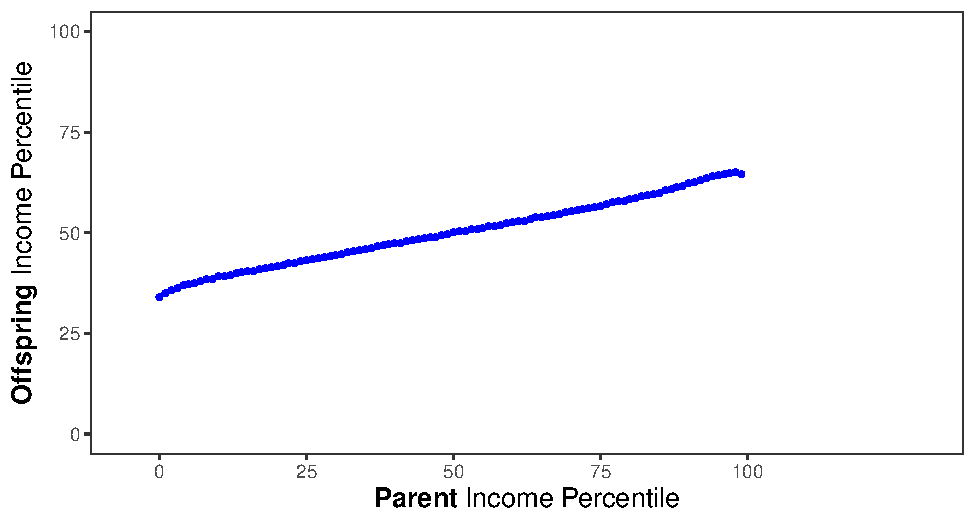
\includegraphics[width = \textwidth]{figures/chetty_figure_1}};
\node<5> at (.5,.4) {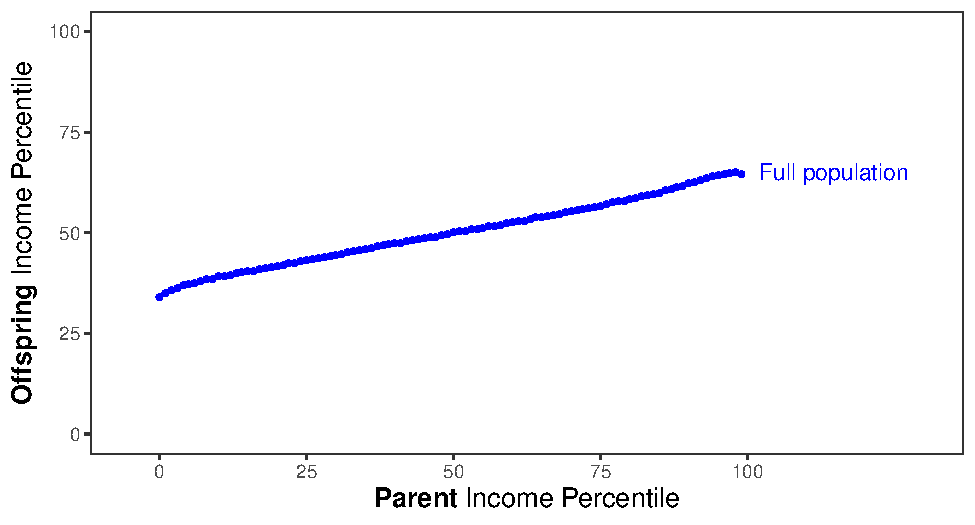
\includegraphics[width = \textwidth]{figures/chetty_figure_2}};
\node<6-8> at (.5,.4) {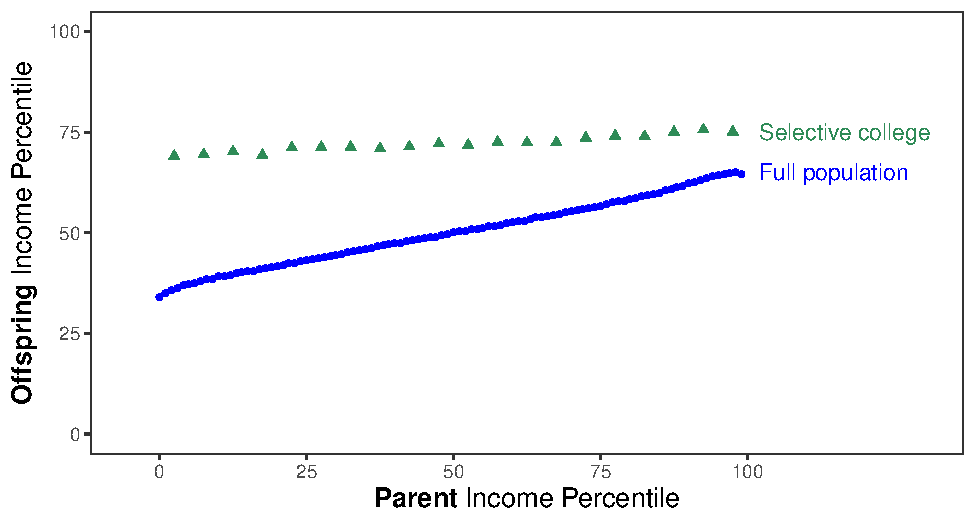
\includegraphics[width = \textwidth]{figures/chetty_figure_3}};
\node<2-8>[anchor = south east, font = {\footnotesize\bf}, color = gray] at (1,.05) {Chetty et al. 2017};
\node<3-4>[anchor = north, font = \small] at (.5,.36) {The average child lands at the};
\node<3-4>[anchor = north west, align = left, font = \scriptsize] at (.1, .3) {\bblue{34th percentile} of income\\if their parents were at\\the \bblue{bottom} of the distribution};
\draw<3-4>[->, thick, blue] (.15,.3) to[bend left] (.15,.34);
\node<4>[anchor = north east, align = right, font = \scriptsize] at (.85, .3) {\bblue{65th percentile} of income\\if their parents were at\\the \bblue{top} of the distribution};
\draw<4>[->, thick, blue] (.83,.4) to[out = 90, in = 350] (.8,.5) to[out = 170, in = 0] (.77, .5);
\draw<7-8>[->, thick, seagreen4] (.173,.4) -- (.173, .51);
\draw<7-8>[->, thick, seagreen4] (.751,.52) -- (.751, .54);
%%%%%%%%
% WESTERN  %
%%%%%%%%
\node<10-13>[align = left, anchor = north west] (western1) at (.2, .6) {The difference in earnings};
\node<10-13>[align = left, anchor = north west] (western2) at (.2, .55) {between blacks and whites};
\node<11-13>[align = left, anchor = north west] (western3) at (.2, .5) {would be reduced only by about 3 percent};
\node<11-13>[align = left, anchor = north west] (western3) at (.2, .45) {if the incarceration rate were zero};
\node<10-13>[anchor = north west] at (.2,.37) {--- Western 2006:12};
\node<10-13>[font = \footnotesize] (race) at (.15, .77) {Race};
\draw<10>[->, line width = 1.2pt, gray] (.2,.53) to[bend left] (race);
\node<11-13>[font = \footnotesize] (earnings) at (.8, .77) {Earnings};
\draw<11>[->, line width = 1.2pt, gray] (.75,.5) to[bend right] (earnings);
\node<12-13>[font = \footnotesize] (incarceration) at (.45, .77) {Incarceration};
\draw<12>[->, line width = 1.2pt, gray] (.2,.43) to[out = 150, in = 200] (incarceration.south west);
%%%%%%%%%%%%%%%%%
% PETERSEN AND MORGAN  %
%%%%%%%%%%%%%%%%%
%\node<14-17>[align = left, anchor = north west] (western1) at (.15, .6) {Suppose sex segregation---by occupation,};
%\node<14-17>[align = left, anchor = north west] (western2) at (.15, .55) {establishment, or occupation-establishment};
%\node<14-17>[align = left, anchor = north west] (western3) at (.15, .5) {---were abolished; what then would the};
%\node<14-17>[align = left, anchor = north west] (western3) at (.15, .45) {remaining gender relative wages be?};
%\node<14-17>[anchor = north west] at (.15,.37) {--- Petersen and Morgan 1995:338};
%\node<15-17>[font = \footnotesize] (gender) at (.15, .77) {Gender};
%\node<16-17>[font = \footnotesize] (occupation) at (.45, .77) {Occupation-Establishment};
%\draw<16>[->, line width = 1.2pt, gray] (.45,.62) -- (occupation);
%\node<17>[font = \footnotesize] (wage) at (.8, .77) {Wage};
%\draw<17>[->, line width = 1.2pt, gray] (.73,.41) to[out = 10, in = 315] (wage);
%%%%%%%%%%%%%%
% We often want to know %
%%%%%%%%%%%%%%
\node<14->[align = left, anchor = west] at (.1,.5) {We often want to know\\if \bblue{intervening} on a treatment variable\\would close gaps};
\node<14>[anchor = south east, gray, align = center, font = \small] at (1,.05) {Jackson \& Vanderweele 2018};
\node<15->[align = left, anchor = west] at (.1,.3) {Would racial disparities in health};
\node<15->[align = left, anchor = west] at (.1,.25) {narrow if we eliminated occupational segregation?};
%\draw<20->[->, line width = 1.2pt, gray] (.6,.54) to[bend right] (.53,.74);
%\node<21->[align = left, anchor = north west, font = \small, gray] (causally) at (.6,.4) {Causally!};
%\draw<21->[->, thick, gray] (causally) -- (.5,.45);
\node<16->[font = \footnotesize] (gender) at (.15, .77) {Race};
\node<17->[font = \footnotesize] (wage) at (.8, .77) {Health};
\node<18->[font = \footnotesize] (occupation) at (.45, .77) {Occupation};
\end{tikzpicture}
\end{frame}

% HAWK'S NEST
\begin{frame}
\begin{tikzpicture}[x = \textwidth, y = \textheight]
\node<1> (image1) at (.5,.5) {\includegraphics[width = \textwidth]{figures/hawks_nest}};
\node<1>[anchor = north east, font = \scriptsize, gray] at (image1.south east) {Image Source: \href{https://en.wikipedia.org/wiki/Hawks\_Nest,\_West\_Virginia\#/media/File:Hawks\_Nest.JPG}{Wikipedia}};
\node<2>[anchor = south] (image2) at (.5,.5) {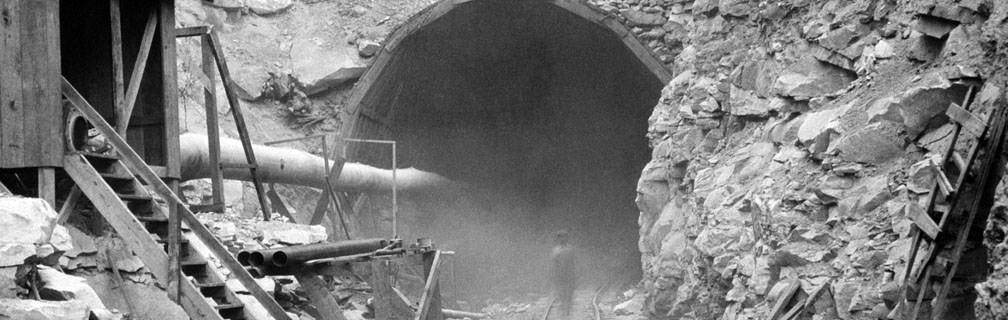
\includegraphics[width = \textwidth]{figures/nps_hawks_nest}};
\node<2>[anchor = north east, font = \scriptsize, gray] at (image2.south east) {Image Source: \href{https://www.nps.gov/neri/planyourvisit/the-hawks-nest-tunnel-disaster-summersville-wv.htm}{National Park Service}};
\end{tikzpicture}
\end{frame}

% PAST WORK ON HEALTH
\begin{frame}
\begin{tikzpicture}[x = \textwidth, y = \textheight]
\node at (0,0) {};
\node at (1,1) {};
\node[anchor = north west, align = left] at (0,.95) {Racial inequality at work affects racial disparities in health};
%\node[anchor = north west] at (0,.9) {The field is only beginning to relate work into health inequities.};
%\node[anchor = north west] at (0,.9) {We know very little about how work relates to health inequities.};
\node<1>[anchor = south east, font = \footnotesize, gray] at (1,.05) {Lipscomb et al.~2006, Ahonen et al.~2018};
\node<2->[anchor = north west, align = center, gray, font = \bf] at (0,.75) {We\\know};
\draw<2->[line width = 2pt, gray, line cap = round] (.125,.8) -- (.125,.55);
\node<3->[anchor = north west] at (.15,.8) {Specific occupations pose substantial hazards};
\node<3->[anchor = north west, font = \small] at (.2,.75) {--- ``Occupational health''};
\node<3>[anchor = south east, font = \footnotesize, gray] at (1,.05) {Buchanan et al. 2010, Lowry et al. 2010, Fleischer et al. 2013, Holmes 2013};
\node<4->[anchor = north west] at (.15,.68) {People of color often hold hazardous occupations};
\node<4>[anchor = south east, font = \footnotesize, gray] at (1,.05) {Chung-Bridges et al.~2008, Fan \& Qian 2017};
\node<5->[anchor = north west] at (.15,.61) {Adjusting for occupation reduces the coefficient on race};
\node<5>[anchor = south east, font = \footnotesize, gray] at (1,.05) {Meyer 2014, Fujishiro et al.~2017};
\node<6->[anchor = north, align = center] at (.2,.45) {These studies \bgreen{describe}\\the world as it exists};
\node<7->[anchor = north, align = center] at (.2,.3) {Disparities\\\bgreen{among} subpopulations};
\node<8->[anchor = north, align = center] at (.8,.45) {They do not \bblue{prescribe}\\how to fix the problem};
\node<9->[anchor = north, align = center] at (.8,.3) {How disparities \bblue{would} change\\if occupations were allocated\\equitably};
\end{tikzpicture}
\end{frame}

% Structure of talk
\begin{frame}
\begin{tikzpicture}[x = \textwidth, y = \textheight]
\node at (0,0) {};
\node at (1,1) {};
\node[anchor = west, align = left] (gce) at (0.2, .9) {The \bblue{gap-closing estimand}:};
\node[anchor = west, align = left] (categories) at (0.2,.85) {The disparity across \bgreen{social categories}};
\node[anchor = west, align = left] (treatment) at (0.2,.8) {that would persist if we \bgreen{equalized a treatment}};
\node[anchor = east, align = right] at (.15, .88) {\bgray{General}};
\node[anchor = east, align = right] at (.15, .83) {\bgray{method}};
\draw[line width = 2pt, gray, line cap = round] (.175,.78) -- (.175,.93);
\node[anchor = west, align = left] (gce) at (.2, .7) {Occupational segregation contributes};
\node[anchor = west, align = left] (categories) at (.2,.65) {to racial disparities in health};
\node[anchor = east, align = right] at (.15, .7) {\bgray{Specific}};
\node[anchor = east, align = right] at (.15, .65) {\bgray{example}};
\draw[line width = 2pt, gray, line cap = round] (.175,.73) -- (.175,.63);
\node (plan) at (.5,.53) {\bgray{Structure of the talk}};
\draw[line width = 2pt, gray, line cap = round] (plan.south west) -- (plan.south east);
\node[anchor = west] at (.04,.44) {\bgray{Introduction}};
\node[anchor = west] at (.04,.38) {\bgray{Data}};
\node[anchor = west] at (.04,.32) {\bgray{Causal Question}};
\node[anchor = west] at (.04,.26) {\bgray{Estimation}};
\node[anchor = west] at (.04,.2) {\bgray{Results}};
\node[anchor = west] at (.04,.14) {\bgray{Broadening out}};
\node[anchor = west] at (.35,.44) {Disparities call for explanations};
\node[anchor = west] at (.35,.38) {Current Population Survey};
\node[anchor = west] at (.35,.32) {How an intervention would close a gap};%change a disparity};
\node[anchor = west] at (.35,.26) {Causal assumptions and predictive tools};
\node[anchor = west] at (.35,.2) {Partially closing a gap in health};
\node[anchor = west] at (.35,.14) {A framework for quantitative methodology};
\draw[->, line width = 2pt, gray] (0,.44) -- (.04, .44);
\end{tikzpicture}
\end{frame}

\section{Data}

% Structure of talk
\begin{frame}
\begin{tikzpicture}[x = \textwidth, y = \textheight]
\node at (0,0) {};
\node at (1,1) {};
\node[anchor = west, align = left] (gce) at (0.2, .9) {The \bblue{gap-closing estimand}:};
\node[anchor = west, align = left] (categories) at (0.2,.85) {The disparity across \bgreen{social categories}};
\node[anchor = west, align = left] (treatment) at (0.2,.8) {that would persist if we \bgreen{equalized a treatment}};
\node[anchor = east, align = right] at (.15, .88) {\bgray{General}};
\node[anchor = east, align = right] at (.15, .83) {\bgray{method}};
\draw[line width = 2pt, gray, line cap = round] (.175,.78) -- (.175,.93);
\node[anchor = west, align = left] (gce) at (.2, .7) {Occupational segregation contributes};
\node[anchor = west, align = left] (categories) at (.2,.65) {to racial disparities in health};
\node[anchor = east, align = right] at (.15, .7) {\bgray{Specific}};
\node[anchor = east, align = right] at (.15, .65) {\bgray{example}};
\draw[line width = 2pt, gray, line cap = round] (.175,.73) -- (.175,.63);
\node (plan) at (.5,.53) {\bgray{Structure of the talk}};
\draw[line width = 2pt, gray, line cap = round] (plan.south west) -- (plan.south east);
\node[anchor = west] at (.04,.44) {\bgray{Introduction}};
\node[anchor = west] at (.04,.38) {\bgray{Data}};
\node[anchor = west] at (.04,.32) {\bgray{Causal Question}};
\node[anchor = west] at (.04,.26) {\bgray{Estimation}};
\node[anchor = west] at (.04,.2) {\bgray{Results}};
\node[anchor = west] at (.04,.14) {\bgray{Broadening out}};
\node[anchor = west] at (.35,.44) {Disparities call for explanations};
\node[anchor = west] at (.35,.38) {Current Population Survey};
\node[anchor = west] at (.35,.32) {How an intervention would close a gap};%change a disparity};
\node[anchor = west] at (.35,.26) {Causal assumptions and predictive tools};
\node[anchor = west] at (.35,.2) {Partially closing a gap in health};
\node[anchor = west] at (.35,.14) {A framework for quantitative methodology};
\draw[->, line width = 2pt, gray] (0,.38) -- (.04, .38);
\end{tikzpicture}
\end{frame}

% MY HEALTH EXAMPLE
\begin{frame}
\label{descriptive_results}
\begin{tikzpicture}[x = \textwidth, y = \textheight]
\node at (0,0) {};
\node at (1,1) {};
\node<1->[anchor = north east, font = \footnotesize, align = right, gray] (note1) at (1,.65) {Current\\Population Survey\\Annual Social and\\Economic Supplement\\Ages 25--60\\2005--2020};
\node<2-17>[anchor = south west, align = left, text width = .87\textwidth, font = \footnotesize, fill = lightgray, fill opacity = .4, text opacity = 1, rounded corners] at (0,.8) {Do you have a health problem or disability which prevents you from working or which limits the kind or amount of work you can do?};
\node<3>[anchor = north west] at (0,.7) {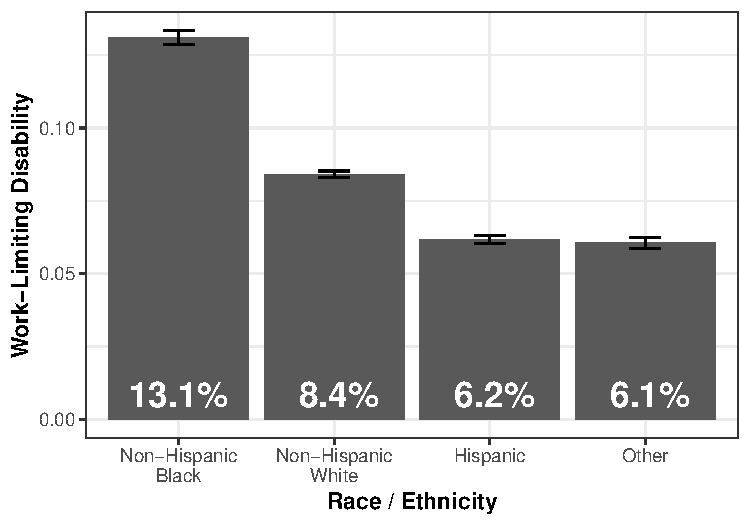
\includegraphics[width = .68\textwidth]{figures/disability_by_race}};
% Timeline
\draw<4-6>[->, gray, line width = 2pt] (0,.5) -- (.65, .5);
\draw<4-6>[thick] (.15,.48) -- (.15, .52);
\draw<4-6>[thick] (.5,.48) -- (.5, .52);
\node<4-6>[anchor = south, font = \footnotesize] at (.15,.52) {Year $y$};
\node<4-6>[anchor = south, font = \footnotesize] at (.5,.52) {Year $y + 1$};
\node<5-6>[anchor = north, font = \footnotesize, align = center] at (.15,.48) {\bgray{Restriction}\\Employed with\\no work-limiting\\disability};
\node<6>[anchor = north, font = \footnotesize, align = center] at (.5,.48) {\bgray{Outcome}\\Onset of\\work-limiting\\disability};
% Onset results
\node<7>[anchor = north west] at (0,.7) {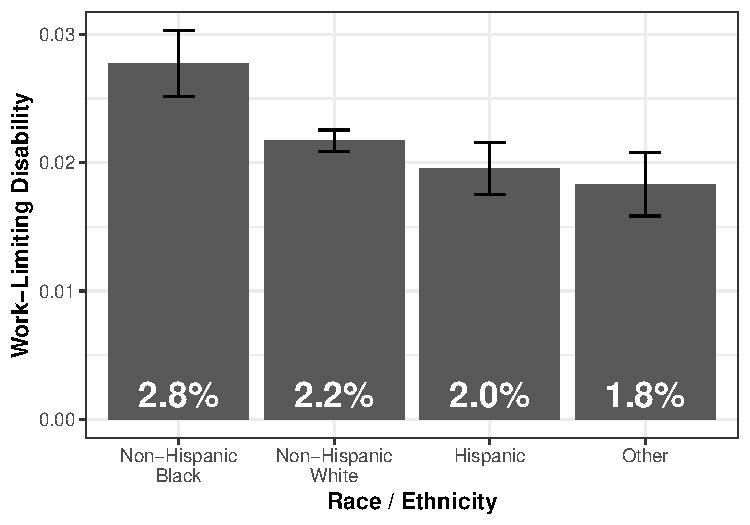
\includegraphics[width = .68\textwidth]{figures/onset_by_race}};
\node<7-18>[anchor = north east, font = \footnotesize, align = right, gray] at (note1.south east) {Employed last year\\No disability\\last year};
\node<7>[anchor = south west, align = left] at (.1,.7) {\textbf{Onset of Work-Limiting Disability}};
\node<8>[anchor = north west] at (0,.7) {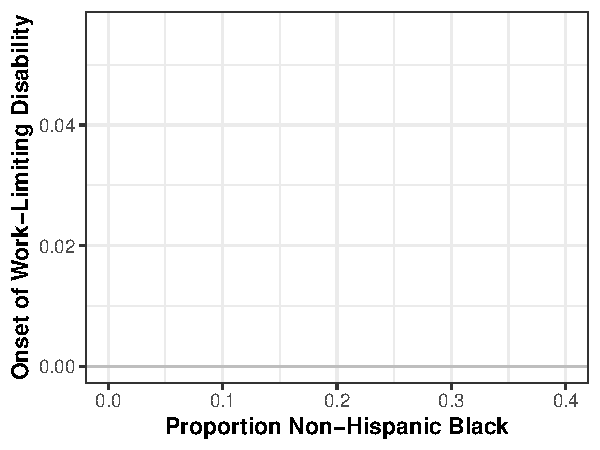
\includegraphics[width = .68\textwidth]{figures/scatter_factual_outcome_re_NonHispanicBlack_slide1}};
\node<9>[anchor = north west] at (0,.7) {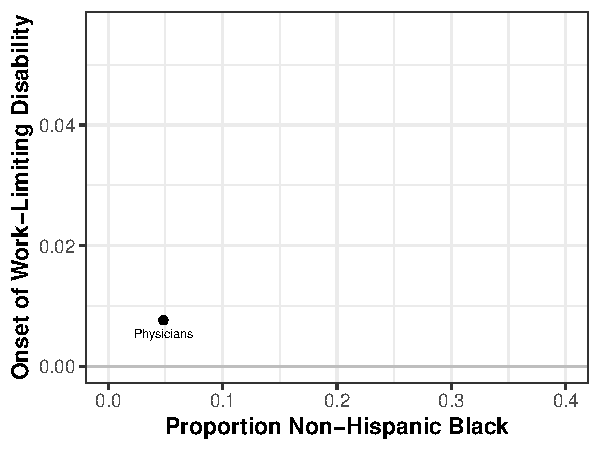
\includegraphics[width = .68\textwidth]{figures/scatter_factual_outcome_re_NonHispanicBlack_slide2}};
\node<10>[anchor = north west] at (0,.7) {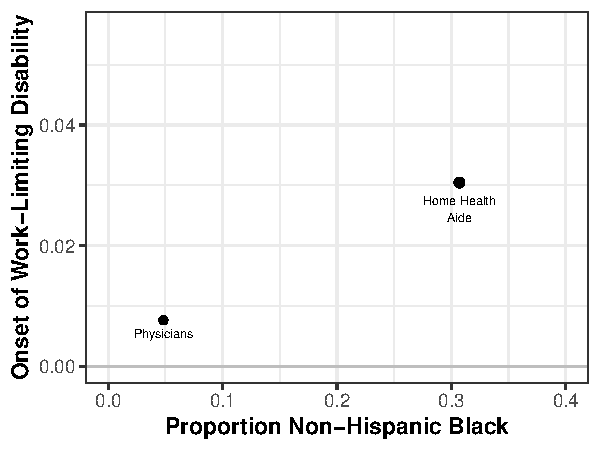
\includegraphics[width = .68\textwidth]{figures/scatter_factual_outcome_re_NonHispanicBlack_slide3}};
\node<11>[anchor = north west] at (0,.7) {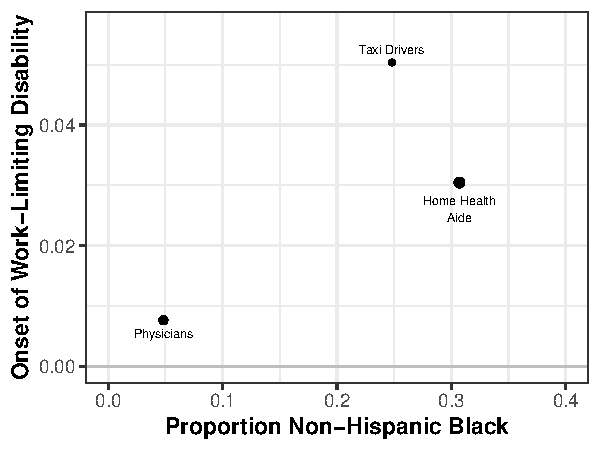
\includegraphics[width = .68\textwidth]{figures/scatter_factual_outcome_re_NonHispanicBlack_slide4}};
\node<12>[anchor = north west] at (0,.7) {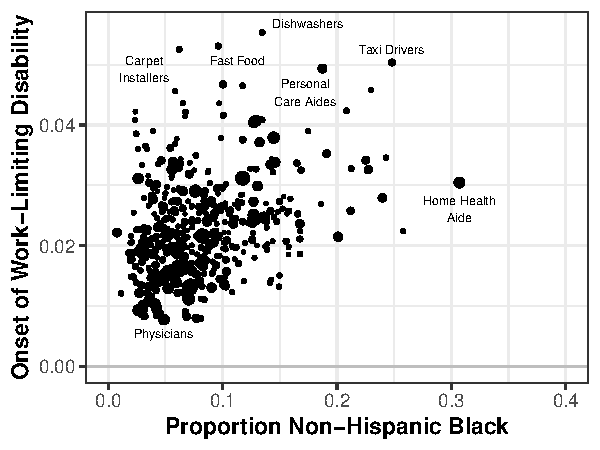
\includegraphics[width = .68\textwidth]{figures/scatter_factual_outcome_re_NonHispanicBlack_slide5}};
\node<13>[anchor = north west] at (0,.7) {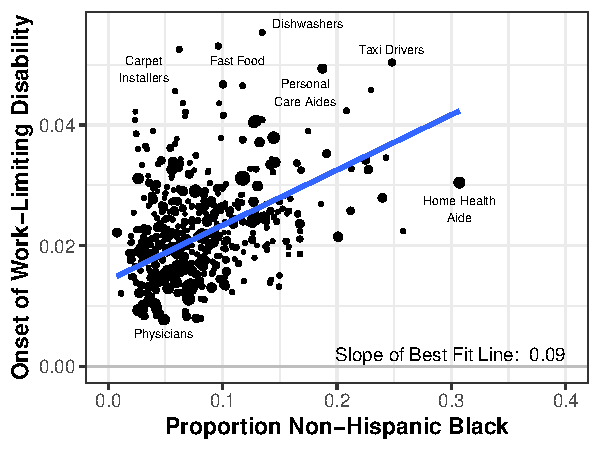
\includegraphics[width = .68\textwidth]{figures/scatter_factual_outcome_re_NonHispanicBlack_slide6}};
\node<14->[anchor = north west] at (0,.7) {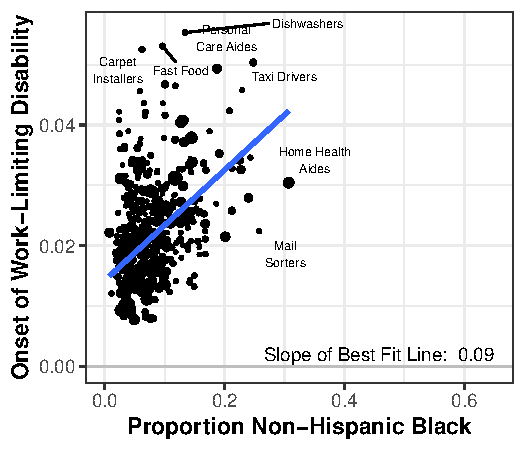
\includegraphics[width = .3\textwidth]{figures/scatter_factual_outcome_re_NonHispanicBlack_annotated}};
\node<15->[anchor = north west] at (0,.4) {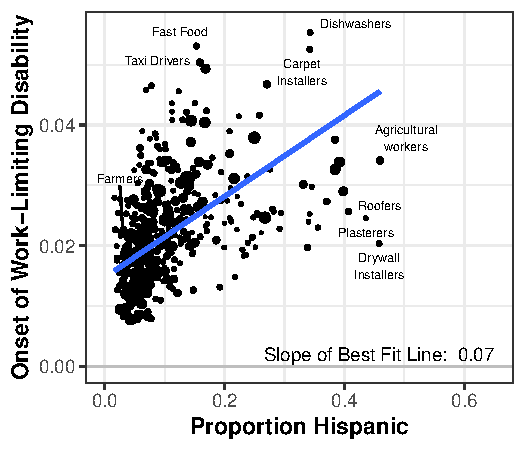
\includegraphics[width = .3\textwidth]{figures/scatter_factual_outcome_re_Hispanic_annotated}};
\node<16->[anchor = north west] at (.35,.7) {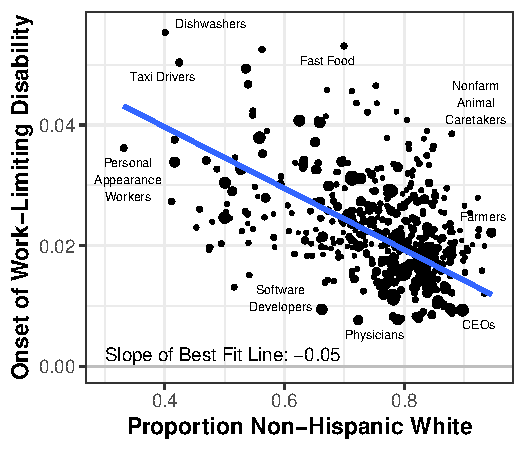
\includegraphics[width = .3\textwidth]{figures/scatter_factual_outcome_re_NonHispanicWhite_annotated}};
\node<17->[anchor = north west] at (.35,.4) {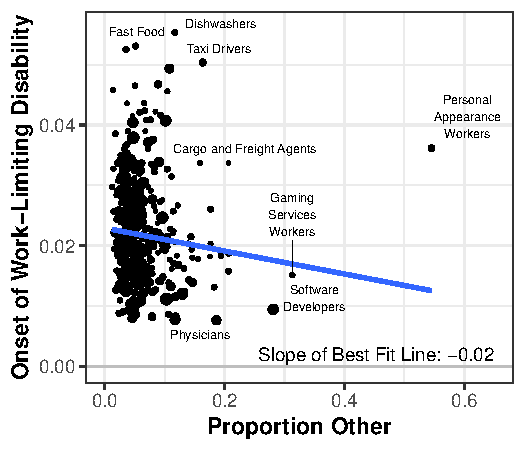
\includegraphics[width = .3\textwidth]{figures/scatter_factual_outcome_re_Other_annotated}};
\node<18>[anchor = south west, align = left] at (0,.8) {To what degree does \bblue{occupational segregation}\\contribute to \bblue{racial health disparities}?};
\end{tikzpicture}
\end{frame}

% Structure of the talk
\begin{frame}
\begin{tikzpicture}[x = \textwidth, y = \textheight]
\node at (0,0) {};
\node at (1,1) {};
\node[anchor = west, align = left] (gce) at (0.2, .9) {The \bblue{gap-closing estimand}:};
\node[anchor = west, align = left] (categories) at (0.2,.85) {The disparity across \bgreen{social categories}};
\node[anchor = west, align = left] (treatment) at (0.2,.8) {that would persist if we \bgreen{equalized a treatment}};
\node[anchor = east, align = right] at (.15, .88) {\bgray{General}};
\node[anchor = east, align = right] at (.15, .83) {\bgray{method}};
\draw[line width = 2pt, gray, line cap = round] (.175,.78) -- (.175,.93);
\node[anchor = west, align = left] (gce) at (.2, .7) {Occupational segregation contributes};
\node[anchor = west, align = left] (categories) at (.2,.65) {to racial disparities in health};
\node[anchor = east, align = right] at (.15, .7) {\bgray{Specific}};
\node[anchor = east, align = right] at (.15, .65) {\bgray{example}};
\draw[line width = 2pt, gray, line cap = round] (.175,.73) -- (.175,.63);
\node (plan) at (.5,.53) {\bgray{Structure of the talk}};
\draw[line width = 2pt, gray, line cap = round] (plan.south west) -- (plan.south east);
\node[anchor = west] at (.04,.44) {\bgray{Introduction}};
\node[anchor = west] at (.04,.38) {\bgray{Data}};
\node[anchor = west] at (.04,.32) {\bgray{Causal Question}};
\node[anchor = west] at (.04,.26) {\bgray{Estimation}};
\node[anchor = west] at (.04,.2) {\bgray{Results}};
\node[anchor = west] at (.04,.14) {\bgray{Broadening out}};
\node[anchor = west] at (.35,.44) {Disparities call for explanations};
\node[anchor = west] at (.35,.38) {Current Population Survey};
\node[anchor = west] at (.35,.32) {How an intervention would close a gap};%change a disparity};
\node[anchor = west] at (.35,.26) {Causal assumptions and predictive tools};
\node[anchor = west] at (.35,.2) {Partially closing a gap in health};
\node[anchor = west] at (.35,.14) {A framework for quantitative methodology};
\draw[->, line width = 2pt, gray] (0,.38) -- (.04, .38);
\end{tikzpicture}
\end{frame}

\section{Causal Question}

% Structure of the talk
\begin{frame}
\begin{tikzpicture}[x = \textwidth, y = \textheight]
\node at (0,0) {};
\node at (1,1) {};
\node[anchor = west, align = left] (gce) at (0.2, .9) {The \bblue{gap-closing estimand}:};
\node[anchor = west, align = left] (categories) at (0.2,.85) {The disparity across \bgreen{social categories}};
\node[anchor = west, align = left] (treatment) at (0.2,.8) {that would persist if we \bgreen{equalized a treatment}};
\node[anchor = east, align = right] at (.15, .88) {\bgray{General}};
\node[anchor = east, align = right] at (.15, .83) {\bgray{method}};
\draw[line width = 2pt, gray, line cap = round] (.175,.78) -- (.175,.93);
\node[anchor = west, align = left] (gce) at (.2, .7) {Occupational segregation contributes};
\node[anchor = west, align = left] (categories) at (.2,.65) {to racial disparities in health};
\node[anchor = east, align = right] at (.15, .7) {\bgray{Specific}};
\node[anchor = east, align = right] at (.15, .65) {\bgray{example}};
\draw[line width = 2pt, gray, line cap = round] (.175,.73) -- (.175,.63);
\node (plan) at (.5,.53) {\bgray{Structure of the talk}};
\draw[line width = 2pt, gray, line cap = round] (plan.south west) -- (plan.south east);
\node[anchor = west] at (.04,.44) {\bgray{Introduction}};
\node[anchor = west] at (.04,.38) {\bgray{Data}};
\node[anchor = west] at (.04,.32) {\bgray{Causal Question}};
\node[anchor = west] at (.04,.26) {\bgray{Estimation}};
\node[anchor = west] at (.04,.2) {\bgray{Results}};
\node[anchor = west] at (.04,.14) {\bgray{Broadening out}};
\node[anchor = west] at (.35,.44) {Disparities call for explanations};
\node[anchor = west] at (.35,.38) {Current Population Survey};
\node[anchor = west] at (.35,.32) {How an intervention would close a gap};%change a disparity};
\node[anchor = west] at (.35,.26) {Causal assumptions and predictive tools};
\node[anchor = west] at (.35,.2) {Partially closing a gap in health};
\node[anchor = west] at (.35,.14) {A framework for quantitative methodology};
\draw[->, line width = 2pt, gray] (0,.32) -- (.04, .32);
\end{tikzpicture}
\end{frame}

% FROM AMONG TO WOULD
\begin{frame}
\begin{tikzpicture}[x = \textwidth, y = .8\textheight]
\node at (.05,-.1) {};
\node at (1,1) {};
\node<1-31>[anchor = north west] at (.05,1.1) {\phantom{From \bgray{among} statements to \bgray{would} statements}};
%\node<25-31>[anchor = north west] at (.05,1.1) {From \bgray{among} statements to \bgray{would} statements};
% Set up the table
\only<2->{
\node[anchor = east, font = \footnotesize] at (.2, .8) {Person 1};
\node[anchor = east, font = \footnotesize] at (.2, .7) {Person 2};
\node[anchor = east, font = \footnotesize] at (.2, .6) {Person 3};
\node[anchor = east, font = \footnotesize] at (.2, .5) {Person 4};
\node[anchor = east, font = \footnotesize] at (.2, .4) {Person 5};
\node[anchor = east, font = \footnotesize] at (.2, .3) {Person 6};
\node[anchor = east, font = \footnotesize] at (.2, .2) {Person 7};
\node[anchor = east, font = \footnotesize] at (.2, .1) {Person 8};
}
\only<3->{
\node[anchor = south, font = \footnotesize, align = center] at (.3, .85) {Administrative\\Assistant};
\node[anchor = south, font = \footnotesize, align = center] at (.5, .85) {Home Health\\Aid};
\node[anchor = south, font = \footnotesize, align = center] at (.7, .85) {Sales\\Supervisor};
}
% Place the factual occupations first
\node<4->[draw, line width = 1pt, circle, fill = lightgray, fill opacity = 1, inner sep = 4pt] (1a) at (.3, .8) {};
\node<5->[draw, line width = 1pt, circle, fill = lightgray, fill opacity = 1, inner sep = 4pt] (2a) at (.3, .7) {};
\node<6->[draw, line width = 1pt, circle, fill = lightgray, fill opacity = 1, inner sep = 4pt] (3b) at (.5, .6) {};
\node<7->[draw, line width = 1pt, circle, fill = lightgray, fill opacity = 1, inner sep = 4pt] (4c) at (.7, .5) {};
\draw<12->[thick, dashed] (.05,.45) -- (.75,.45);
\node<8->[draw, line width = 1pt, diamond, fill = lightgray, fill opacity = 1, inner sep = 4pt] (5b) at (.5, .4) {};
\node<9->[draw, line width = 1pt, diamond, fill = lightgray, fill opacity = 1, inner sep = 4pt] (6c) at (.7, .3) {};
\node<10->[draw, line width = 1pt, diamond, fill = lightgray, fill opacity = 1, inner sep = 4pt] (7b) at (.5, .2) {};
\node<11->[draw, line width = 1pt, diamond, fill = lightgray, fill opacity = 1, inner sep = 4pt] (8a) at (.3, .1) {};
% Create the legend for sick and healthy
\only<13-28>{
\node[anchor = west, font = \bf] at (.9,.5) {Legend};
\draw[thick] (.8,.05) -- (.8,.55) -- (1.1,.55);
\node[anchor = east] at (.9,.4) {\textcolor{seagreen4}{$\checkmark$}};
\node[anchor = east] at (.9,.3) {
\includegraphics[width = 10pt]{figures/injury}};
\node[anchor = west] at (.9,.4) {Healthy};
\node[anchor = west] at (.9,.3) {Sick};
}
% Place the health conditions on those
\node<14->[seagreen4] at (1a) {$\checkmark$};
\node<15->[seagreen4] at (2a) {$\checkmark$};
\node<16-> at (3b) {
\includegraphics[width = 10pt]{figures/injury}};
\only<17->{
\node[seagreen4] at (4c) {$\checkmark$};
\node at (5b) {
\includegraphics[width = 10pt]{figures/injury}};
\node[seagreen4] at (6c) {$\checkmark$};
\node at (7b) {
\includegraphics[width = 10pt]{figures/injury}};
\node at (8a) {
\includegraphics[width = 10pt]{figures/injury}};
}
% Do the total disparity
\node<18-19>[red, font = \bf, draw, line width = 2pt, rounded corners] at (.6,.75) {1 / 4 sick};
\node<19>[red, font = \bf, draw, line width = 2pt, rounded corners] at (.6, .1) {3 / 4 sick};
%\node<18>[red, font = \bf, align = center] at (.95, .75) {Descriptive\\Disparity\\$\frac{3}{4}-\frac{1}{4}=50\%$};
% Do the conditional disparity
\draw<20-21>[fill = lightgray, fill opacity = .2] (.4,.05) rectangle (.6,.98);
\node<21>[anchor = north, align = center, font = \footnotesize] at (.5,.05) {No disparity \bgray{among}\\home health aids};
%\draw<20>[fill = lightgray, fill opacity = .2] (.6,.05) rectangle (.8,.98);
%\node<20>[anchor = north, align = center, font = \footnotesize] at (.7,.05) {No disparity \bgray{among}\\sales supervisors};
%\draw<21>[fill = lightgray, fill opacity = .2] (.2,.05) rectangle (.4,.98);
%\node<21>[anchor = north, align = center, font = \footnotesize] at (.3,.05) {Disparity \bgray{among}\\administrative assistants};
% Begin causal with row 1
\node<23->[circle, fill = lightgray, fill opacity = 1, inner sep = 4pt] (1b) at (.5, .8) {};
\node<24-> at (1b) {
\includegraphics[width = 10pt]{figures/injury}};
%\node<26-28>[font = \footnotesize, align = left, anchor = west] at (.83, .95) {Occupation\\\bgray{contributes}\\to health.};
%\node<27-28>[font = \footnotesize, align = left, anchor = west] at (.83, .7) {Person 1 \bgray{would}\\have different health\\in a different\\occupation.};
% Create the legend for observed and unobserved
\only<25-28>{
\node[anchor = east, draw, line width = 1pt, diamond, fill = lightgray, fill opacity = 1, inner sep = 4pt] (obsDiamond) at (.9,.2) {};
\node[anchor = east, draw, line width = 1pt, circle, fill = lightgray, fill opacity = 1, inner sep = 4pt] (obsCircle) at (obsDiamond.west) {};
\node[anchor = west] at (.9,.2) {Observed};
\node[anchor = east, diamond, fill = lightgray, fill opacity = 1, inner sep = 4pt] (unobsDiamond) at (.9,.1) {};
\node[anchor = east, circle, fill = lightgray, fill opacity = 1, inner sep = 4pt] (unobsCircle) at (unobsDiamond.west) {};
\node[anchor = west] at (.9,.1) {Unobserved};
\node[anchor = south east, gray] at (1.1,-.07) {Imbens and Rubin 2015};
}
\node<26->[circle, fill = lightgray, fill opacity = 1, inner sep = 4pt] (1c) at (.7, .8) {};
\node<26->[seagreen4] at (1c) {$\checkmark$};
% Add person 2 counterfactuals
\only<27->{
\node[circle, fill = lightgray, fill opacity = 1, inner sep = 4pt] (2b) at (.5, .7) {};
\node[circle, fill = lightgray, fill opacity = 1, inner sep = 4pt] (2c) at (.7, .7) {};
\node[seagreen4] at (2b) {$\checkmark$};
\node[seagreen4] at (2c) {$\checkmark$};
}
% Add all others' counterfactuals
\only<28->{
\node[circle, fill = lightgray, fill opacity = 1, inner sep = 4pt] (3a) at (.3, .6) {};
\node[circle, fill = lightgray, fill opacity = 1, inner sep = 4pt] (3c) at (.7, .6) {};
\node at (3a) {
\includegraphics[width = 10pt]{figures/injury}};
\node[seagreen4] at (3c) {$\checkmark$};
\node[circle, fill = lightgray, fill opacity = 1, inner sep = 4pt] (4a) at (.3, .5) {};
\node[circle, fill = lightgray, fill opacity = 1, inner sep = 4pt] (4b) at (.5, .5) {};
\node[seagreen4] at (4a) {$\checkmark$};
\node[seagreen4] at (4b) {$\checkmark$};
\node[diamond, fill = lightgray, fill opacity = 1, inner sep = 4pt] (5a) at (.3, .4) {};
\node[diamond, fill = lightgray, fill opacity = 1, inner sep = 4pt] (5c) at (.7, .4) {};
\node[seagreen4] at (5a) {$\checkmark$};
\node[seagreen4] at (5c) {$\checkmark$};
\node[diamond, fill = lightgray, fill opacity = 1, inner sep = 4pt] (6a) at (.3, .3) {};
\node[diamond, fill = lightgray, fill opacity = 1, inner sep = 4pt] (6b) at (.5, .3) {};
\node[seagreen4] at (6a) {$\checkmark$};
\node at (6b) {
\includegraphics[width = 10pt]{figures/injury}};
\node[diamond, fill = lightgray, fill opacity = 1, inner sep = 4pt] (7a) at (.3, .2) {};
\node[diamond, fill = lightgray, fill opacity = 1, inner sep = 4pt] (7c) at (.7, .2) {};
\node at (7a) {
\includegraphics[width = 10pt]{figures/injury}};
\node[seagreen4] at (7c) {$\checkmark$};
\node[diamond, fill = lightgray, fill opacity = 1, inner sep = 4pt] (8b) at (.5, .1) {};
\node at (8b) {
\includegraphics[width = 10pt]{figures/injury}};
\node[diamond, fill = lightgray, fill opacity = 1, inner sep = 4pt] (8c) at (.7, .1) {};
\node[seagreen4] at (8c) {$\checkmark$};
}
% AFTER 31, LEGEND IS GONE
% STOCHASTIC TREATMENT BEGINS
\node<29->[anchor = north west] at (.05,1.1) {What if occupations were \bgray{assigned at random}?};
% Average for each circle
\node<30-38>[font = {\footnotesize\bf}, anchor = south, align = center] at (.87,.85) {Probability\\of Sickness};
\node<31-38> at (.87,.8) {1 / 3};
\node<32-38> at (.87,.7) {0 / 3};
\node<33-38> at (.87,.6) {2 / 3};
\node<34-38> at (.87,.5) {0 / 3};
% Average for each diamond
\node<35-38> at (.87,.4) {1 / 3};
\node<35-38> at (.87,.3) {1 / 3};
\node<35-38> at (.87,.2) {2 / 3};
\node<35-38> at (.87,.1) {2 / 3};
% Average for all circles
\node<36-38>[draw, circle] at (1,.65) {$\frac{3}{12}$};
% Average for all diamonds
\node<37-38>[draw, diamond, inner sep = 2pt] at (1,.25) {$\frac{6}{12}$};
% Difference
\node<38->[anchor = east, font = {\footnotesize\bf}, gray] at (.6, .02) {Counterfactual Disparity:};
\only<38->{
\node[draw, diamond, inner sep = 0pt, font = \footnotesize] at (.65,.02) {$\frac{6}{12}$};
\node[font = \footnotesize] at (.725,.02) {$-$};
\node[draw, circle, inner sep = 0pt, font = \footnotesize] at (.8,.02) {$\frac{3}{12}$};
\node[anchor = west, font = \footnotesize] at (.85,.02) {$=\frac{3}{12}$};
\node[anchor = west, font = \footnotesize] at (.95,.02) {$=25\%$};
}
\node<39->[anchor = east, font = {\footnotesize\bf}, gray] at (.6, -.07) {Factual Disparity:};
\only<39->{
\node[draw, diamond, inner sep = 0pt, font = \footnotesize] at (.65,-.07) {$\frac{3}{4}$};
\node[font = \footnotesize] at (.725,-.07) {$-$};
\node[draw, circle, inner sep = 0pt, font = \footnotesize] at (.8,-.07) {$\frac{1}{4}$};
\node[anchor = west, font = \footnotesize] at (.85,-.07) {$=\frac{1}{2}$};
\node[anchor = west, font = \footnotesize] at (.95,-.07) {$=50\%$};
}
\only<39->{
	\node[circle, fill = white, draw = white, inner sep = 4pt] at (1b) {};
	\node[circle, fill = white, draw = white, inner sep = 4pt] at (1c) {};
	\node[circle, fill = white, draw = white, inner sep = 4pt] at (2b) {};
	\node[circle, fill = white, draw = white, inner sep = 4pt] at (2c) {};
	\node[circle, fill = white, draw = white, inner sep = 4pt] at (3a) {};
	\node[circle, fill = white, draw = white, inner sep = 4pt] at (3c) {};
	\node[circle, fill = white, draw = white, inner sep = 4pt] at (4a) {};
	\node[circle, fill = white, draw = white, inner sep = 4pt] at (4b) {};
	\node[diamond, fill = white, draw = white, inner sep = 4pt] at (5a) {};
	\node[diamond, fill = white, draw = white, inner sep = 4pt] at (5c) {};
	\node[diamond, fill = white, draw = white, inner sep = 4pt] at (6a) {};
	\node[diamond, fill = white, draw = white, inner sep = 4pt] at (6b) {};
	\node[diamond, fill = white, draw = white, inner sep = 4pt] at (7a) {};
	\node[diamond, fill = white, draw = white, inner sep = 4pt] at (7c) {};
	\node[diamond, fill = white, draw = white, inner sep = 4pt] at (8b) {};
	\node[diamond, fill = white, draw = white, inner sep = 4pt] at (8c) {};
}
\node<40>[anchor = north, align = center] at (.95,.65) {Assigning\\occupations\\at random\\would cut\\the disparity\\in \bblue{half!}};
\draw<40>[->, line width = 2pt, blue] (1,.25) -- (1,.1);
\end{tikzpicture}
\end{frame}

% EQUITABLE ASSIGNMENT RULE
\begin{frame}
\label{assignment_rules}
    \begin{tikzpicture}[x = \textwidth, y = \textheight]
    \node at (0,0) {};
    \node at (1,1) {};
    \node<1-8>[anchor = north west] at (0,.95) {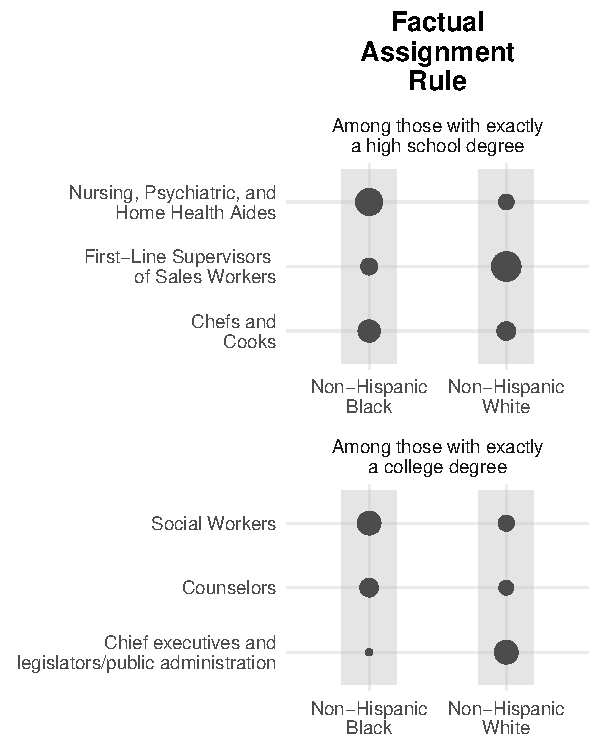
\includegraphics[height = .7\textheight]{figures/pi_bucket_factual}};
    \draw<1>[white, fill = white] (.37,.53) rectangle (.5,.785);
    \draw<3-8>[->, gray, line width = 2pt] (.57,.685) -- (.67,.685);
    \node<3-8>[align = center, font = \footnotesize] (equalize) at (.62,.59) {Equalize\\occupational\\assignment};
    \node<4->[anchor = north east] at (1,.95) {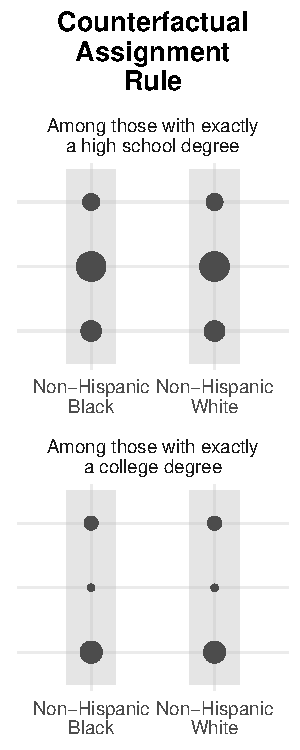
\includegraphics[height = .7\textheight]{figures/pi_bucket_counterfactual_noLabels}};
    \draw<1-5>[white, fill = white] (0,0) rectangle (1,.53);
    \node<5-8>[align = center, anchor = north, font = \footnotesize] at (equalize.south) {within\\education};
    \draw<6-8>[->, gray, line width = 2pt] (.57,.385) -- (.67,.385);
    \node<7-8>[anchor = north west] (equitable) at (0,.15) {Equalizing within education is \bblue{equitable}};
    \node<8>[anchor = north west] at (equitable.north east) {but also \bblue{realistic}};
    \end{tikzpicture}
\end{frame}

\begin{frame}
\begin{tikzpicture}[x = \textwidth, y = \textheight]
\node at (0,0) {};
\node at (1,1) {};
\node<2->[anchor = north west, align = left] at (0,.9) {We now have a way to think about what \bblue{would} happen\\if occupations were \bblue{assigned differently}};
\node<3->[anchor = north west] at (0,.7) {We have a way to think about \bblue{equitable assignment} to occupations};
\node<4->[anchor = north west, align = left] at (0,.55) {But that seems to suggest a \bred{grand claim}:\\what would happen under a structural intervention\\to desegregate occupations};
%\node<5>[anchor = north, font = \Large, red] at (.5,.35) {Is that right?};
% Begin science table reminder
\only<2>{
\node[anchor = east, font = \footnotesize] at (.2, .45) {Person 1};
\node[anchor = east, font = \footnotesize] at (.2, .4) {Person 2};
\node[anchor = east, font = \footnotesize] at (.2, .35) {Person 3};
\node[anchor = east, font = \footnotesize] at (.2, .3) {Person 4};
\node[anchor = east, font = \footnotesize] at (.2, .25) {Person 5};
\node[anchor = east, font = \footnotesize] at (.2, .2) {Person 6};
\node[anchor = east, font = \footnotesize] at (.2, .15) {Person 7};
\node[anchor = east, font = \footnotesize] at (.2, .1) {Person 8};
\node[anchor = south, font = \footnotesize, align = center] at (.3, .5) {Administrative\\Assistant};
\node[anchor = south, font = \footnotesize, align = center] at (.5, .5) {Home Health\\Aid};
\node[anchor = south, font = \footnotesize, align = center] at (.7, .5) {Sales\\Supervisor};
\node[draw, line width = 1pt, circle, fill = lightgray, fill opacity = 1, inner sep = 3pt] (1a) at (.3, .45) {};
\node[draw, line width = 1pt, circle, fill = lightgray, fill opacity = 1, inner sep = 3pt] (2a) at (.3, .4) {};
\node[draw, line width = 1pt, circle, fill = lightgray, fill opacity = 1, inner sep = 3pt] (3b) at (.5, .35) {};
\node[draw, line width = 1pt, circle, fill = lightgray, fill opacity = 1, inner sep = 3pt] (4c) at (.7, .3) {};
\draw[thick, dashed] (.05,.275) -- (.75,.275);
\node[draw, line width = 1pt, diamond, fill = lightgray, fill opacity = 1, inner sep = 3pt] (5b) at (.5, .25) {};
\node[draw, line width = 1pt, diamond, fill = lightgray, fill opacity = 1, inner sep = 3pt] (6c) at (.7, .2) {};
\node[draw, line width = 1pt, diamond, fill = lightgray, fill opacity = 1, inner sep = 3pt] (7b) at (.5, .15) {};
\node[draw, line width = 1pt, diamond, fill = lightgray, fill opacity = 1, inner sep = 3pt] (8a) at (.3, .1) {};
\node[circle, fill = lightgray, fill opacity = 1, inner sep = 3pt] (3a) at (.3, .35) {};
\node[circle, fill = lightgray, fill opacity = 1, inner sep = 3pt] (4a) at (.3, .3) {};
\node[diamond, fill = lightgray, fill opacity = 1, inner sep = 3pt] (5a) at (.3, .25) {};
\node[diamond, fill = lightgray, fill opacity = 1, inner sep = 3pt] (6a) at (.3, .2) {};
\node[diamond, fill = lightgray, fill opacity = 1, inner sep = 3pt] (7a) at (.3, .15) {};
\node[circle, fill = lightgray, fill opacity = 1, inner sep = 3pt] (1b) at (.5, .45) {};
\node[circle, fill = lightgray, fill opacity = 1, inner sep = 3pt] (2b) at (.5, .4) {};
\node[circle, fill = lightgray, fill opacity = 1, inner sep = 3pt] (4b) at (.5, .3) {};
\node[diamond, fill = lightgray, fill opacity = 1, inner sep = 3pt] (6b) at (.5, .2) {};
\node[diamond, fill = lightgray, fill opacity = 1, inner sep = 3pt] (8b) at (.5, .1) {};
\node[circle, fill = lightgray, fill opacity = 1, inner sep = 3pt] (1c) at (.7, .45) {};
\node[circle, fill = lightgray, fill opacity = 1, inner sep = 3pt] (2c) at (.7, .4) {};
\node[circle, fill = lightgray, fill opacity = 1, inner sep = 3pt] (3c) at (.7, .35) {};
\node[diamond, fill = lightgray, fill opacity = 1, inner sep = 3pt] (5c) at (.7, .25) {};
\node[diamond, fill = lightgray, fill opacity = 1, inner sep = 3pt] (7c) at (.7, .15) {};
\node[diamond, fill = lightgray, fill opacity = 1, inner sep = 3pt] (8c) at (.7, .1) {};
\node[font = \tiny] at (1b) {?};
\node[font = \tiny] at (1c) {?};
\node[font = \tiny] at (2b) {?};
\node[font = \tiny] at (2c) {?};
\node[font = \tiny] at (3a) {?};
\node[font = \tiny] at (3c) {?};
\node[font = \tiny] at (4a) {?};
\node[font = \tiny] at (4b) {?};
\node[font = \tiny] at (5a) {?};
\node[font = \tiny] at (5c) {?};
\node[font = \tiny] at (6a) {?};
\node[font = \tiny] at (6b) {?};
\node[font = \tiny] at (7a) {?};
\node[font = \tiny] at (7c) {?};
\node[font = \tiny] at (8b) {?};
\node[font = \tiny] at (8c) {?};
}
% Begin equitable rule reminder
\node<3>[anchor = north] at (.5,.63) {\resizebox{\textwidth}{!}{
    \begin{tikzpicture}[x = \textwidth, y = \textheight]
    \node at (0,0) {};
    \node at (1,1) {};
    \node[anchor = north west] at (0,.95) {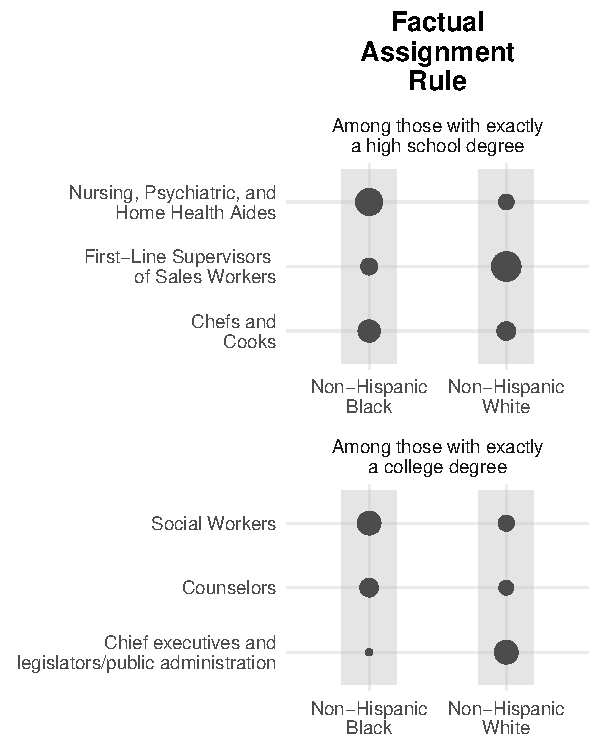
\includegraphics[height = .7\textheight]{figures/pi_bucket_factual}};
    \draw[->, gray, line width = 2pt] (.57,.685) -- (.67,.685);
    %\node[align = center, font = \footnotesize] (equalize) at (.62,.59) {Equalize\\occupational\\assignment};
    \node[anchor = north east] at (1,.95) {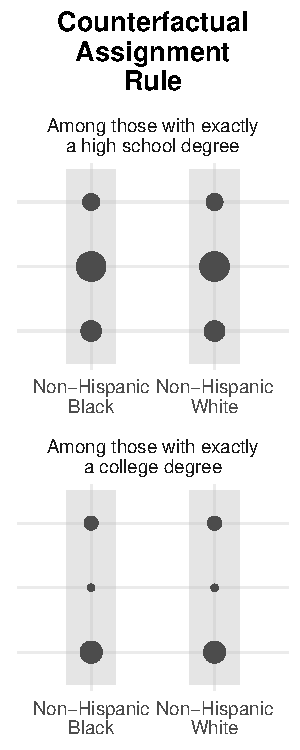
\includegraphics[height = .7\textheight]{figures/pi_bucket_counterfactual_noLabels}};
    \draw[white, fill = white] (0,0) rectangle (1,.53);
    \end{tikzpicture}}};
\end{tikzpicture}
\end{frame}

% NEW SCOPE SLIDE
\begin{frame}
\begin{tikzpicture}[x = \textwidth, y = \textheight]
\node at (0,0) {};
\node at (1,1) {};
\node<1-6,12->[anchor = north west, align = left, font = \small, text width = \textwidth, text badly ragged] at (0, .55) {Black-white pay gap ``if the incarceration rate were zero.''\\--- Western (2006:127)};
\node<2-6,12->[anchor = north west, align = left, font = \small, text width = \textwidth, text badly ragged] at (0, .42) {Class origin pay gap in ``a utopian world of `college for all'.''\\--- Zhou (2019:466).};
\node<3-6,12->[anchor = north west, align = left, font = \small, text width = \textwidth, text badly ragged] at (0, .29) {Sex pay gap if ``sex segregation...were abolished.''\\--- Petersen and Morgan (1995:338).};
\node<4->[anchor = south] at (.25,.9) {Global interpretation};
\node<4->[anchor = south, align = center, gray, font = \small] at (.25,.75) {Equalize for\\\textbf{everyone}\\at once};
\node<5>[anchor = south east, align = right, font = \small, gray] at (1, .05) {Link \& Phelan 1995, Raftery \& Hout 1993, Lucas 2001};
\node<6->[anchor = south] at (.75,.9) {Local interpretation};
\node<6->[anchor = south, align = center, gray, font = \small] (local_interpretation) at (.75,.75) {Equalize for\\\textbf{one unit}\\at a time};
% BEGIN LOCAL ILLUSTRATION
\node<7-11>[anchor = south east, font = \footnotesize, gray, align = right] at (1,.1) {Hern\'an \&\\Robins 2016};
\node<7-11>[anchor = south, gray, font = \bf] (target_trial) at (.42,.6) {Target Trial};
\draw<7-11>[rounded corners, line width = 2pt, gray] (.02,.1) rectangle (.82,.6);
\draw<7-11>[->, line width = 1.2pt, gray] (local_interpretation) to[bend right] (target_trial);
\only<8-11>{
\draw[thick, rounded corners] (.12, .45) rectangle (.32,.55);
\node (local_set_i) at (.22, .45) {};
\node[diamond, fill = lightgray, draw = lightgray, font = \footnotesize, inner sep = 2pt] at (.17, .5) {};
\node[diamond, fill = lightgray, draw = lightgray, font = \footnotesize, inner sep = 2pt] at (.22, .5) {};
\node[diamond, fill = lightgray, draw = lightgray, font = \footnotesize, inner sep = 2pt] at (.27, .5) {};
% Non-Hispanic Black
\draw[thick, rounded corners] (.52, .45) rectangle (.72,.55);
\node (local_set_j) at (.62, .45) {};
\node[circle, fill = lightgray, draw = lightgray, font = \footnotesize, inner sep = 2pt] at (.57, .5) {};
\node[circle, fill = lightgray, draw = lightgray, font = \footnotesize, inner sep = 2pt] at (.62, .5) {};
\node[circle, fill = lightgray, draw = lightgray, font = \footnotesize, inner sep = 2pt] at (.67, .5) {};
}
% Suppose you took 1 person per category
\only<9-11>{
\node[align = center, font = \footnotesize] at (.42,.35) {Assign treatment\\to 1 person per category};
\node[diamond, fill = lightgray, draw = lightgray, font = \footnotesize, inner sep = 2pt] (local_i) at (.22, .35) {};
\node[circle, fill = lightgray, draw = lightgray, font = \footnotesize, inner sep = 2pt] (local_j) at (.62, .35) {};
\draw<2->[->, thick] (local_set_i) -- (local_i);
\draw<2->[->, thick] (local_set_j) -- (local_j);
}
\node<10-11>[anchor = south, font = \footnotesize, align = center] at (.42,.2) {See the resulting disparity};
\node<11>[anchor = south, font = \footnotesize, align = center] at (.42,.1) {Average over many hypothetical repetitions};
% TENSION
\draw<13->[line width = 2.5pt] (.25,.7) -- (.75, .7);
\node<13->[font = \Huge] at (.25,.7) {$\bullet$};
\node<13->[font = \Huge] at (.75,.7) {$\bullet$};
\node<13->[anchor = south, align = center, font = {\small\bf}] at (.5,.7) {Tension};
\node<13->[anchor = east, align = right, font = \small] at (1,.7) {Most\\empirically\\credible};
\node<13->[anchor = west, align = left, font = \small] at (0,.7) {Least\\empirically\\credible};
\node<14>[anchor = north, align = right, font = \footnotesize, gray] at (.3,.65) {Policy-relevant?};
\draw<14>[->, thick, gray] (.3,.65) -- (.3,.69);
\node<15>[anchor = north, align = right, font = \footnotesize, gray] at (.7,.65) {Policy-relevant.};
\draw<15>[->, thick, gray] (.7,.65) -- (.7,.69);
\end{tikzpicture}
\end{frame}

% Structure of the talk
\begin{frame}
\begin{tikzpicture}[x = \textwidth, y = \textheight]
\node at (0,0) {};
\node at (1,1) {};
\node[anchor = west, align = left] (gce) at (0.2, .9) {The \bblue{gap-closing estimand}:};
\node[anchor = west, align = left] (categories) at (0.2,.85) {The disparity across \bgreen{social categories}};
\node[anchor = west, align = left] (treatment) at (0.2,.8) {that would persist if we \bgreen{equalized a treatment}};
\node[anchor = east, align = right] at (.15, .88) {\bgray{General}};
\node[anchor = east, align = right] at (.15, .83) {\bgray{method}};
\draw[line width = 2pt, gray, line cap = round] (.175,.78) -- (.175,.93);
\node[anchor = west, align = left] (gce) at (.2, .7) {Occupational segregation contributes};
\node[anchor = west, align = left] (categories) at (.2,.65) {to racial disparities in health};
\node[anchor = east, align = right] at (.15, .7) {\bgray{Specific}};
\node[anchor = east, align = right] at (.15, .65) {\bgray{example}};
\draw[line width = 2pt, gray, line cap = round] (.175,.73) -- (.175,.63);
\node (plan) at (.5,.53) {\bgray{Structure of the talk}};
\draw[line width = 2pt, gray, line cap = round] (plan.south west) -- (plan.south east);
\node[anchor = west] at (.04,.44) {\bgray{Introduction}};
\node[anchor = west] at (.04,.38) {\bgray{Data}};
\node[anchor = west] at (.04,.32) {\bgray{Causal Question}};
\node[anchor = west] at (.04,.26) {\bgray{Estimation}};
\node[anchor = west] at (.04,.2) {\bgray{Results}};
\node[anchor = west] at (.04,.14) {\bgray{Broadening out}};
\node[anchor = west] at (.35,.44) {Disparities call for explanations};
\node[anchor = west] at (.35,.38) {Current Population Survey};
\node[anchor = west] at (.35,.32) {How an intervention would close a gap};%change a disparity};
\node[anchor = west] at (.35,.26) {Causal assumptions and predictive tools};
\node[anchor = west] at (.35,.2) {Partially closing a gap in health};
\node[anchor = west] at (.35,.14) {A framework for quantitative methodology};
\draw[->, line width = 2pt, gray] (0,.32) -- (.04, .32);
\end{tikzpicture}
\end{frame}

\section{Estimation}

% Structure of the talk
\begin{frame}
\begin{tikzpicture}[x = \textwidth, y = \textheight]
\node at (0,0) {};
\node at (1,1) {};
\node[anchor = west, align = left] (gce) at (0.2, .9) {The \bblue{gap-closing estimand}:};
\node[anchor = west, align = left] (categories) at (0.2,.85) {The disparity across \bgreen{social categories}};
\node[anchor = west, align = left] (treatment) at (0.2,.8) {that would persist if we \bgreen{equalized a treatment}};
\node[anchor = east, align = right] at (.15, .88) {\bgray{General}};
\node[anchor = east, align = right] at (.15, .83) {\bgray{method}};
\draw[line width = 2pt, gray, line cap = round] (.175,.78) -- (.175,.93);
\node[anchor = west, align = left] (gce) at (.2, .7) {Occupational segregation contributes};
\node[anchor = west, align = left] (categories) at (.2,.65) {to racial disparities in health};
\node[anchor = east, align = right] at (.15, .7) {\bgray{Specific}};
\node[anchor = east, align = right] at (.15, .65) {\bgray{example}};
\draw[line width = 2pt, gray, line cap = round] (.175,.73) -- (.175,.63);
\node (plan) at (.5,.53) {\bgray{Structure of the talk}};
\draw[line width = 2pt, gray, line cap = round] (plan.south west) -- (plan.south east);
\node[anchor = west] at (.04,.44) {\bgray{Introduction}};
\node[anchor = west] at (.04,.38) {\bgray{Data}};
\node[anchor = west] at (.04,.32) {\bgray{Causal Question}};
\node[anchor = west] at (.04,.26) {\bgray{Estimation}};
\node[anchor = west] at (.04,.2) {\bgray{Results}};
\node[anchor = west] at (.04,.14) {\bgray{Broadening out}};
\node[anchor = west] at (.35,.44) {Disparities call for explanations};
\node[anchor = west] at (.35,.38) {Current Population Survey};
\node[anchor = west] at (.35,.32) {How an intervention would close a gap};%change a disparity};
\node[anchor = west] at (.35,.26) {Causal assumptions and predictive tools};
\node[anchor = west] at (.35,.2) {Partially closing a gap in health};
\node[anchor = west] at (.35,.14) {A framework for quantitative methodology};
\draw[->, line width = 2pt, gray] (0,.26) -- (.04, .26);
\end{tikzpicture}
\end{frame}

\begin{frame}
\label{dag}
\begin{tikzpicture}[x = \textwidth, y = \textheight]
\node at (0,0) {};
\node at (1,1) {};
\node[anchor = north west, align = left] at (0,.95) {\bblue{Identification:}};
\node[anchor = north west, align = left] at (.25,.95) {We have to impute the outcome each person $i$\\would realize in each occupation $t$};
\node<2>[anchor = east, align = left, font = \small, gray] at (1,.1) {Pearl 2009, Morgan \& Winship 2015, Hern\'an \& Robins 2020};
\node<2,4-> (l) at (.3,.5) {$\vec{L}$};
\node<3>[draw, rounded corners] (l) at (.3,.5) {$\vec{L}$};
\node<2,4-> (x) at (.3,.7) {Race};
\node<3>[draw, rounded corners] (x) at (.3,.7) {Race};
\node<2-> (t) at (.5,.6) {Occupation};
\node<2-> (y) at (.75,.6) {Health};
\node<2->[anchor = north, font = \footnotesize, align = center] at (l.south west) {Predictors};
\draw<2->[->, thick] (l) -- (t);
\draw<2->[->, thick] (l) to[bend right = 15] (y);
\draw<2->[->, line width = 2pt, blue] (t) -- (y);
\draw<2-7,9->[->, thick] (x) -- (t);
\draw<2-7,9->[->, thick] (x) -- (l);
\draw<2-7,9->[->, thick] (x) to[bend left = 40] (y);
% Confounding of T is bad
\node<4,11>[red] (u) at (.5,.4) {$U$};
\draw<4,11>[->, red, line width = 2pt] (u) -- (t);
\draw<4,11>[->, red, line width = 2pt] (u) to[bend right = 20] (y); 
% Confounding of X is ok
\node<5>[seagreen4] (v) at (.15,.4) {$V$};
\draw<5>[->, seagreen4, line width = 2pt] (v) to[bend left = 20] (x);
\draw<5>[->, seagreen4, line width = 2pt] (v) to[out = 0, in = 240] (y); 
% Agnostic about causal effect of X
\node<6-9>[anchor = west, align = left] at (0,.35) {A gap-closing estimand is \bblue{agnostic} about the causal effect of race};
\node<7-9>[anchor = west, align = left, font = \small] at (0,.28) {--- Race can affect everything};
\node<8-9>[anchor = west, align = left, font = \small] at (0,.22) {--- Race can have no causal effects};
\node<9>[anchor = west, align = left, font = \small] at (0,.16) {--- The effect of race can be philosophically complex};
\node<7>[anchor = east, align = left, font = \small, gray] at (1,.1) {Williams et al. 2019};
\node<8>[anchor = east, align = left, font = \small, gray] at (1,.1) {Greiner \& Rubin 2011};
\node<9>[anchor = east, align = left, font = \small, gray] at (1,.1) {Sen \& Wasow 2016, Kohler-Hausmann 2018};
\end{tikzpicture}
\end{frame}

\begin{frame}
\label{data}
\begin{tikzpicture}[x = \textwidth, y = \textheight]
\node at (0,0) {};
\node at (1,1) {};
\node[anchor = west] at (0,.95) {\bblue{Data} Linked Current Population Survey, 2005--2020};
\draw[->, line width = 2pt, gray] (0,.8) -- (1,.8);
\draw[thick] (.15,.78) -- (.15,.82);
\draw[thick] (.75,.78) -- (.75,.82);
\node[anchor = south, align = center, font = \footnotesize] at (.15,.82) {March\\Year $y$};
\node[anchor = south, align = center, font = \footnotesize] at (.75,.82) {March\\Year $y+1$};
\node<2->[anchor = north, align = center, font = \footnotesize] (outcome) at (.75,.78) {Outcome};
\node<2->[anchor = south, align = center, font = {\small\bf}, gray] (disability) at (.75,.59) {Onset of\\work-limiting disability};
\draw<2->[thick] (disability) -- (outcome);
\node<2->[anchor = north east, align = left, text width = .5\textwidth, font = \small, fill = lightgray, fill opacity = .4, text opacity = 1, rounded corners] at (1,.59) {Do you have a health problem or disability which prevents you from working or which limits the kind or amount of work you can do?};
\node<3->[anchor = north, align = center, font = \footnotesize] (lags) at (.15,.78) {Covariates\\Occupation};
% Sample restrictions
\node<4->[anchor = north west, align = left, font = \small] (restricted) at (0,.65) {\bgray{Sample restriction:}\\Employed with no\\work-limiting disability};
\draw<4->[thick] (lags) -- (.15,.65);
% Predictors
\node<5->[anchor = north west, font = \small] at (0,.5) {\bgray{Predictors:}};
\node<5->[anchor = north west, align = left, font = \footnotesize] at (0,.46) {Race, Sex\\Education\\Foreign born};
\node<5->[anchor = north west, align = left, font = \footnotesize] at (.2,.46) {Self-rated health\\Age\\Year};
% Assessment of credibility
\node<6-19>[anchor = north west, font = \small] at (0,.325) {\bblue{Credibility Check:}};
\node<7-19>[anchor = east, font = \footnotesize] at (.55,.2) {Woman 1};
\node<7-19>[anchor = east, font = \footnotesize] at (.55,.1) {Woman 2};
\node<7-19>[anchor = south, font = \footnotesize, align = center] at (.65,.25) {Administrative\\Assistant};
\node<7-19>[anchor = south, font = \footnotesize, align = center] at (.85,.25) {Home Health\\Aid};
\node<7-19>[diamond, fill = lightgray, draw = black, inner sep = 4pt] (1a) at (.65,.2) {};
\node<7-19>[diamond, fill = lightgray, draw = black, inner sep = 4pt] (2b) at (.85,.1) {};
\node<8-19>[anchor = north west, align = left, font = \footnotesize] at (0,.275) {Both Black};
\node<9-19>[anchor = north west, align = left, font = \footnotesize] at (0,.235) {Both high school graduates};
\node<10-19>[anchor = north west, align = left, font = \footnotesize] at (0,.195) {Neither foreign born};
\node<11-19>[anchor = north west, align = left, font = \footnotesize] at (0,.155) {Both report excellent health};
\node<12-19>[anchor = north west, align = left, font = \footnotesize] at (0,.115) {Both 30 years old in 2010};
\node<13-19>[seagreen4] at (1a) {$\checkmark$};
\node<14-19> at (2b) {
\includegraphics[width = 10pt]{figures/injury}};
\node<15-19>[diamond, fill = lightgray, draw = lightgray, line width = 1pt, inner sep = 4pt] (1b) at (.85,.2) {};
\node<15-19>[diamond, fill = lightgray, draw = lightgray, line width = 1pt, inner sep = 4pt] (2a) at (.65,.1) {};
\draw<16-19>[->, thick] (2b) to node[midway, right]  {?} (1b);
\node<17-19>[seagreen4] at (1b) {
\includegraphics[width = 10pt]{figures/injury}};
\draw<18-19>[->, thick] (1a) to node[midway, left]  {?} (2a);
\node<19>[seagreen4] at (2a) {$\checkmark$};
% Supplemental restrictions
\node<20->[anchor = north west] at (0,.3) {\bgray{Supplemental restrictions:}};
\node<21->[anchor = south west, font = \footnotesize] (difficulties) at (0,.18) {\textbf{No difficulty with}};
\node<21->[anchor = north west, font = \footnotesize, align = left] at (0,.2) {hearing\\vision\\remembering};
\node<21->[anchor = north west, font = \footnotesize, align = left] at (.2,.2) {walking\\performing basic duties\\caring for personal needs};
\node<22->[anchor = west, font = \footnotesize, align = left] at (.55,.13) {\textbf{and}};
\node<22->[anchor = west, font = \footnotesize, align = left] at (.65,.13) {Never left a job\\for health reasons};
\end{tikzpicture}
\end{frame}

% NEW HOW TO ESTIMATE
\begin{frame}
\begin{tikzpicture}[x = \textwidth, y = \textheight]
\node at (0,0) {};
\node at (1,1) {};
\node[anchor = north] (how) at (.5, .95) {How to estimate a gap-closing estimand};
\draw[line width = 2pt, gray, line cap = rounded] (how.south west) -- (how.south east);
% Some shading boxes that appear later
% but are coded here so that text appears on top of them
\draw<18-20>[fill = lightgray, fill opacity = .5, rounded corners, draw = lightgray] (0,.425) rectangle (1,.475);
\draw<21>[fill = lightgray, fill opacity = .5, rounded corners, draw = lightgray] (0,.375) rectangle (1,.425);
\draw<22>[fill = lightgray, fill opacity = .5, rounded corners, draw = lightgray] (0,.325) rectangle (1,.375);
\draw<23>[fill = lightgray, fill opacity = .5, rounded corners, draw = lightgray] (0,.275) rectangle (1,.325);
\draw<24>[fill = lightgray, fill opacity = .5, rounded corners, draw = lightgray] (0,.225) rectangle (1,.275);
\draw<25>[fill = lightgray, fill opacity = .5, rounded corners, draw = lightgray] (0,.175) rectangle (1,.225);
\draw<26>[fill = lightgray, fill opacity = .5, rounded corners, draw = lightgray] (0,.125) rectangle (1,.175);
\draw<27>[fill = lightgray, fill opacity = .5, rounded corners, draw = lightgray] (0,.075) rectangle (1,.125);
\draw<29>[fill = lightgray, fill opacity = .5, rounded corners, draw = lightgray] (.85,.275) rectangle (.95,.475);
\draw<31>[fill = lightgray, fill opacity = .5, rounded corners, draw = lightgray] (.85,.075) rectangle (.95,.275);
\only<2->{
% Begin science table
\node[anchor = east, font = \footnotesize] at (.2, .45) {Person 1};
\node[anchor = east, font = \footnotesize] at (.2, .4) {Person 2};
\node[anchor = east, font = \footnotesize] at (.2, .35) {Person 3};
\node[anchor = east, font = \footnotesize] at (.2, .3) {Person 4};
\node[anchor = east, font = \footnotesize] at (.2, .25) {Person 5};
\node[anchor = east, font = \footnotesize] at (.2, .2) {Person 6};
\node[anchor = east, font = \footnotesize] at (.2, .15) {Person 7};
\node[anchor = east, font = \footnotesize] at (.2, .1) {Person 8};
\node[anchor = south, font = \footnotesize, align = center] at (.3, .5) {Administrative\\Assistant};
\node[anchor = south, font = \footnotesize, align = center] at (.5, .5) {Home Health\\Aid};
\node[anchor = south, font = \footnotesize, align = center] at (.7, .5) {Sales\\Supervisor};
% Factual occupations first
\node[draw, line width = 1pt, circle, fill = lightgray, fill opacity = 1, inner sep = 3pt] (1a) at (.3, .45) {};
\node[draw, line width = 1pt, circle, fill = lightgray, fill opacity = 1, inner sep = 3pt] (2a) at (.3, .4) {};
\node[draw, line width = 1pt, circle, fill = lightgray, fill opacity = 1, inner sep = 3pt] (3b) at (.5, .35) {};
\node[draw, line width = 1pt, circle, fill = lightgray, fill opacity = 1, inner sep = 3pt] (4c) at (.7, .3) {};
\draw[thick, dashed] (.05,.275) -- (.75,.275);
\node[draw, line width = 1pt, diamond, fill = lightgray, fill opacity = 1, inner sep = 3pt] (5b) at (.5, .25) {};
\node[draw, line width = 1pt, diamond, fill = lightgray, fill opacity = 1, inner sep = 3pt] (6c) at (.7, .2) {};
\node[draw, line width = 1pt, diamond, fill = lightgray, fill opacity = 1, inner sep = 3pt] (7b) at (.5, .15) {};
\node[draw, line width = 1pt, diamond, fill = lightgray, fill opacity = 1, inner sep = 3pt] (8a) at (.3, .1) {};
}
% Counterfactual occupations
\only<2,9->{
\node[circle, fill = lightgray, fill opacity = 1, inner sep = 3pt] (3a) at (.3, .35) {};
\node[circle, fill = lightgray, fill opacity = 1, inner sep = 3pt] (4a) at (.3, .3) {};
\node[diamond, fill = lightgray, fill opacity = 1, inner sep = 3pt] (5a) at (.3, .25) {};
\node[diamond, fill = lightgray, fill opacity = 1, inner sep = 3pt] (6a) at (.3, .2) {};
\node[diamond, fill = lightgray, fill opacity = 1, inner sep = 3pt] (7a) at (.3, .15) {};
}
\only<2,12->{
\node[circle, fill = lightgray, fill opacity = 1, inner sep = 3pt] (1b) at (.5, .45) {};
\node[circle, fill = lightgray, fill opacity = 1, inner sep = 3pt] (2b) at (.5, .4) {};
\node[circle, fill = lightgray, fill opacity = 1, inner sep = 3pt] (4b) at (.5, .3) {};
\node[diamond, fill = lightgray, fill opacity = 1, inner sep = 3pt] (6b) at (.5, .2) {};
\node[diamond, fill = lightgray, fill opacity = 1, inner sep = 3pt] (8b) at (.5, .1) {};
}
\only<2,15->{
\node[circle, fill = lightgray, fill opacity = 1, inner sep = 3pt] (1c) at (.7, .45) {};
\node[circle, fill = lightgray, fill opacity = 1, inner sep = 3pt] (2c) at (.7, .4) {};
\node[circle, fill = lightgray, fill opacity = 1, inner sep = 3pt] (3c) at (.7, .35) {};
\node[diamond, fill = lightgray, fill opacity = 1, inner sep = 3pt] (5c) at (.7, .25) {};
\node[diamond, fill = lightgray, fill opacity = 1, inner sep = 3pt] (7c) at (.7, .15) {};
\node[diamond, fill = lightgray, fill opacity = 1, inner sep = 3pt] (8c) at (.7, .1) {};
}
% Counterfactual question marks
\only<2>{
\node[font = \tiny] at (1b) {?};
\node[font = \tiny] at (1c) {?};
\node[font = \tiny] at (2b) {?};
\node[font = \tiny] at (2c) {?};
\node[font = \tiny] at (3a) {?};
\node[font = \tiny] at (3c) {?};
\node[font = \tiny] at (4a) {?};
\node[font = \tiny] at (4b) {?};
\node[font = \tiny] at (5a) {?};
\node[font = \tiny] at (5c) {?};
\node[font = \tiny] at (6a) {?};
\node[font = \tiny] at (6b) {?};
\node[font = \tiny] at (7a) {?};
\node[font = \tiny] at (7c) {?};
\node[font = \tiny] at (8b) {?};
\node[font = \tiny] at (8c) {?};
}
% Begin prediction function
\node<4-16>[draw = gray, line width = 1.2pt, rounded corners, align = center] at (.5,.73) {Prediction\\Function};
\node<5-16>[anchor = south] (input) at (.2,.78) {Input};
\draw<5-16>[thick] (input.south west) -- (input.south east);
\node<5-6,16>[font = \footnotesize, align = center, anchor = north] at (.2,.78) {$\text{Covariates}_i$\\$\text{Occupation}_i$};
\draw<5-16>[->, thick] (.3,.73) -- (.37,.73);
\node<6-16>[anchor = south] (output) at (.8,.78) {Output};
\draw<6-16>[thick] (output.south west) -- (output.south east);
\node<6-16>[font = \footnotesize, align = center, anchor = north] (predicted) at (.8,.78) {Predicted\\$\text{Health}_i$};
\draw<6-16>[->, thick] (.63,.73) -- (.7,.73);
% Make the input administrative assistant
\node<7-9>[font = \footnotesize, align = center, anchor = north] at (.2,.78) {$\text{Covariates}_i$\\$\substack{\texttt{Administrative}\\\texttt{Assistant}}$};
\node<8-9>[font = \footnotesize, align = center, anchor = west] at (predicted.east) {$\left(\substack{\text{as an}\\\texttt{Administrative}\\\texttt{Assistant}}\right)$};
\only<9->{
\node[font = \tiny] at (1a) {$\hat{y}$};
\node[font = \tiny] at (2a) {$\hat{y}$};
\node[font = \tiny] at (3a) {$\hat{y}$};
\node[font = \tiny] at (4a) {$\hat{y}$};
\node[font = \tiny] at (5a) {$\hat{y}$};
\node[font = \tiny] at (6a) {$\hat{y}$};
\node[font = \tiny] at (7a) {$\hat{y}$};
\node[font = \tiny] at (8a) {$\hat{y}$};
}
% Make the input home health aid
\node<10-12>[font = \footnotesize, align = center, anchor = north] at (.2,.78) {$\text{Covariates}_i$\\$\substack{\texttt{Home Health}\\\texttt{Aid}}$};
\node<11-12>[font = \footnotesize, align = center, anchor = west] at (predicted.east) {$\left(\substack{\text{as a}\\\texttt{Home Health}\\\texttt{Aid}}\right)$};
\only<12->{
\node[font = \tiny] at (1b) {$\hat{y}$};
\node[font = \tiny] at (2b) {$\hat{y}$};
\node[font = \tiny] at (3b) {$\hat{y}$};
\node[font = \tiny] at (4b) {$\hat{y}$};
\node[font = \tiny] at (5b) {$\hat{y}$};
\node[font = \tiny] at (6b) {$\hat{y}$};
\node[font = \tiny] at (7b) {$\hat{y}$};
\node[font = \tiny] at (8b) {$\hat{y}$};
}
% Make the input sales supervisor
\node<13-15>[font = \footnotesize, align = center, anchor = north] at (.2,.78) {$\text{Covariates}_i$\\$\substack{\texttt{Sales}\\\texttt{Supervisor}}$};
\node<14-15>[font = \footnotesize, align = center, anchor = west] at (predicted.east) {$\left(\substack{\text{as a}\\\texttt{Sales}\\\texttt{Supervisor}}\right)$};
\only<15->{
\node[font = \tiny] at (1c) {$\hat{y}$};
\node[font = \tiny] at (2c) {$\hat{y}$};
\node[font = \tiny] at (3c) {$\hat{y}$};
\node[font = \tiny] at (4c) {$\hat{y}$};
\node[font = \tiny] at (5c) {$\hat{y}$};
\node[font = \tiny] at (6c) {$\hat{y}$};
\node[font = \tiny] at (7c) {$\hat{y}$};
\node[font = \tiny] at (8c) {$\hat{y}$};
}
\node<16>[font = \small, anchor = south east, gray, align = right] at (1,.1) {Robins 1986\\Hahn 1998};
\node<19->[anchor = south, font = \footnotesize, align = center] at (.9,.5) {Probability\\of Disability\\in an Equitable\\Occupation Lottery};
\node<20-29> at (.9,.45) {0.02};
\node<21-29> at (.9,.4) {0.01};
\node<22-29> at (.9,.35) {0.02};
\node<23-29> at (.9,.3) {0.03};
\node<24-31> at (.9,.25) {0.02};
\node<25-31> at (.9,.2) {0.03};
\node<26-31> at (.9,.15) {0.04};
\node<27-31> at (.9,.1) {0.03};
\node<30->[circle, fill = lightgray, draw = lightgray] at (.9,.375) {0.02};
\node<32->[diamond, fill = lightgray, draw = lightgray] at (.9,.175) {0.03};
\only<33>{
\node[anchor = north west] at (.25, .85) {1) Learn a prediction function};
\node[anchor = north west] at (.25, .8) {2) Predict counterfactuals};
\node[anchor = north west] at (.25, .75) {3) Aggregate to an estimate};
}
\end{tikzpicture}
\end{frame}

% Structure of the talk
\begin{frame}
\begin{tikzpicture}[x = \textwidth, y = \textheight]
\node at (0,0) {};
\node at (1,1) {};
\node[anchor = west, align = left] (gce) at (0.2, .9) {The \bblue{gap-closing estimand}:};
\node[anchor = west, align = left] (categories) at (0.2,.85) {The disparity across \bgreen{social categories}};
\node[anchor = west, align = left] (treatment) at (0.2,.8) {that would persist if we \bgreen{equalized a treatment}};
\node[anchor = east, align = right] at (.15, .88) {\bgray{General}};
\node[anchor = east, align = right] at (.15, .83) {\bgray{method}};
\draw[line width = 2pt, gray, line cap = round] (.175,.78) -- (.175,.93);
\node[anchor = west, align = left] (gce) at (.2, .7) {Occupational segregation contributes};
\node[anchor = west, align = left] (categories) at (.2,.65) {to racial disparities in health};
\node[anchor = east, align = right] at (.15, .7) {\bgray{Specific}};
\node[anchor = east, align = right] at (.15, .65) {\bgray{example}};
\draw[line width = 2pt, gray, line cap = round] (.175,.73) -- (.175,.63);
\node (plan) at (.5,.53) {\bgray{Structure of the talk}};
\draw[line width = 2pt, gray, line cap = round] (plan.south west) -- (plan.south east);
\node[anchor = west] at (.04,.44) {\bgray{Introduction}};
\node[anchor = west] at (.04,.38) {\bgray{Data}};
\node[anchor = west] at (.04,.32) {\bgray{Causal Question}};
\node[anchor = west] at (.04,.26) {\bgray{Estimation}};
\node[anchor = west] at (.04,.2) {\bgray{Results}};
\node[anchor = west] at (.04,.14) {\bgray{Broadening out}};
\node[anchor = west] at (.35,.44) {Disparities call for explanations};
\node[anchor = west] at (.35,.38) {Current Population Survey};
\node[anchor = west] at (.35,.32) {How an intervention would close a gap};%change a disparity};
\node[anchor = west] at (.35,.26) {Causal assumptions and predictive tools};
\node[anchor = west] at (.35,.2) {Partially closing a gap in health};
\node[anchor = west] at (.35,.14) {A framework for quantitative methodology};
\draw[->, line width = 2pt, gray] (0,.26) -- (.04, .26);
\end{tikzpicture}
\end{frame}

\section{Results}

% Structure of the talk
\begin{frame}
\begin{tikzpicture}[x = \textwidth, y = \textheight]
\node at (0,0) {};
\node at (1,1) {};
\node[anchor = west, align = left] (gce) at (0.2, .9) {The \bblue{gap-closing estimand}:};
\node[anchor = west, align = left] (categories) at (0.2,.85) {The disparity across \bgreen{social categories}};
\node[anchor = west, align = left] (treatment) at (0.2,.8) {that would persist if we \bgreen{equalized a treatment}};
\node[anchor = east, align = right] at (.15, .88) {\bgray{General}};
\node[anchor = east, align = right] at (.15, .83) {\bgray{method}};
\draw[line width = 2pt, gray, line cap = round] (.175,.78) -- (.175,.93);
\node[anchor = west, align = left] (gce) at (.2, .7) {Occupational segregation contributes};
\node[anchor = west, align = left] (categories) at (.2,.65) {to racial disparities in health};
\node[anchor = east, align = right] at (.15, .7) {\bgray{Specific}};
\node[anchor = east, align = right] at (.15, .65) {\bgray{example}};
\draw[line width = 2pt, gray, line cap = round] (.175,.73) -- (.175,.63);
\node (plan) at (.5,.53) {\bgray{Structure of the talk}};
\draw[line width = 2pt, gray, line cap = round] (plan.south west) -- (plan.south east);
\node[anchor = west] at (.04,.44) {\bgray{Introduction}};
\node[anchor = west] at (.04,.38) {\bgray{Data}};
\node[anchor = west] at (.04,.32) {\bgray{Causal Question}};
\node[anchor = west] at (.04,.26) {\bgray{Estimation}};
\node[anchor = west] at (.04,.2) {\bgray{Results}};
\node[anchor = west] at (.04,.14) {\bgray{Broadening out}};
\node[anchor = west] at (.35,.44) {Disparities call for explanations};
\node[anchor = west] at (.35,.38) {Current Population Survey};
\node[anchor = west] at (.35,.32) {How an intervention would close a gap};%change a disparity};
\node[anchor = west] at (.35,.26) {Causal assumptions and predictive tools};
\node[anchor = west] at (.35,.2) {Partially closing a gap in health};
\node[anchor = west] at (.35,.14) {A framework for quantitative methodology};
\draw[->, line width = 2pt, gray] (0,.2) -- (.04, .2);
\end{tikzpicture}
\end{frame}

\begin{frame}
\label{results}
\begin{center}
\onslide<5->{Occupational segregation is \bblue{partially responsible} for\\the Black-white disparity in work-limiting disability}
\end{center}
\begin{tikzpicture}[x = \textwidth]
    \node<1>[anchor = west] at (0,0) {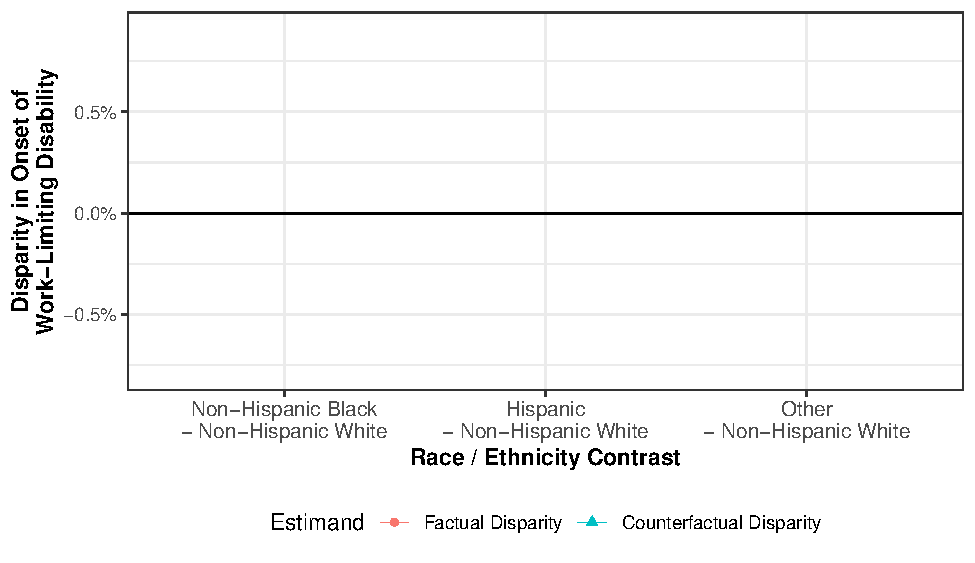
\includegraphics[width = \textwidth]{figures/disparity_1}};
    \node<2>[anchor = west] at (0,0) {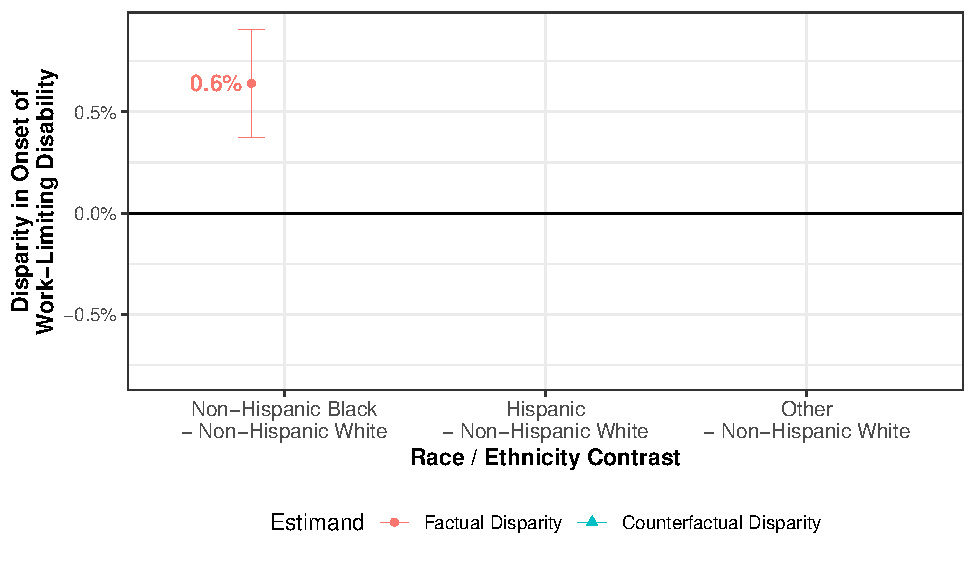
\includegraphics[width = \textwidth]{figures/disparity_2}};
    \node<3-5>[anchor = west] at (0,0) {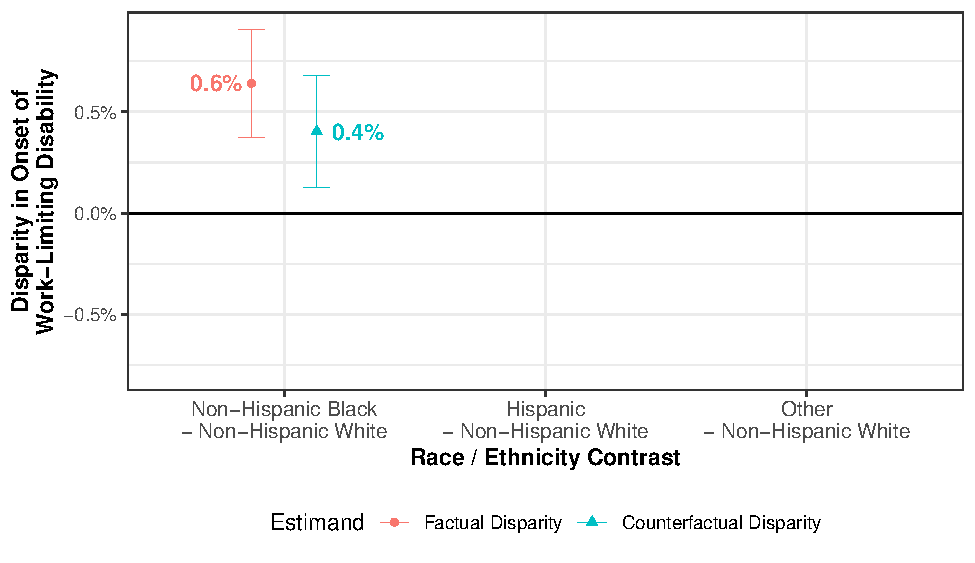
\includegraphics[width = \textwidth]{figures/disparity_3}};
    \node<6>[anchor = west] at (0,0) {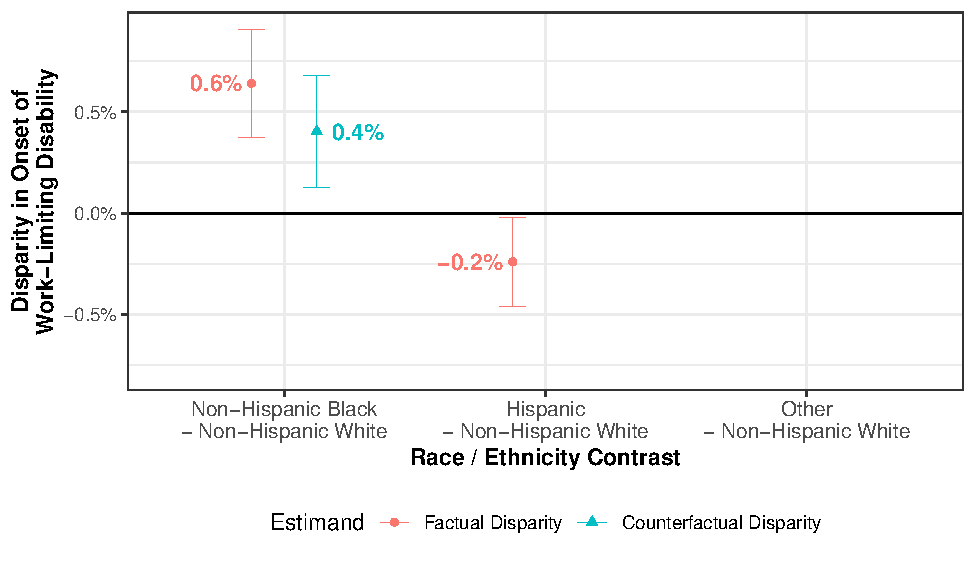
\includegraphics[width = \textwidth]{figures/disparity_4}};
    \node<7-8>[anchor = west] at (0,0) {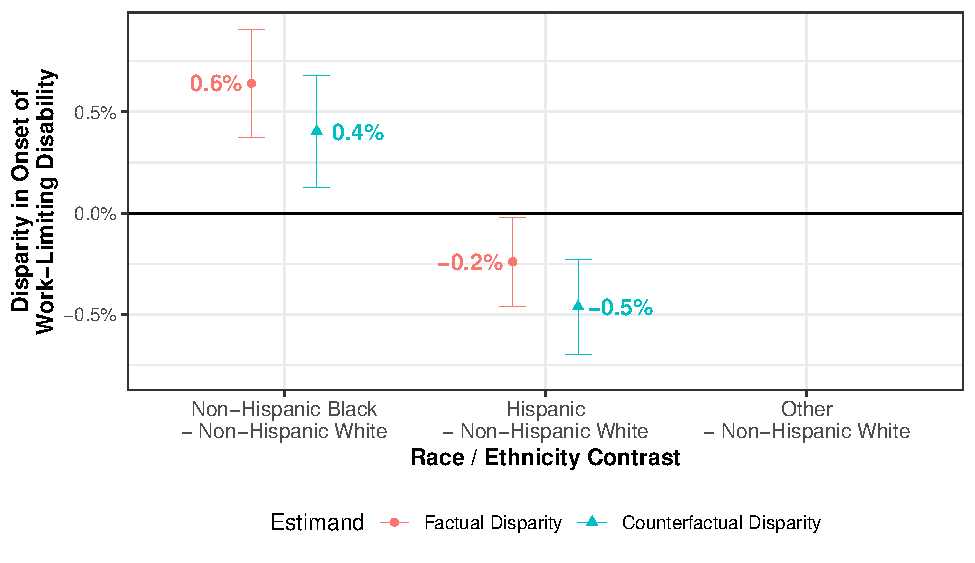
\includegraphics[width = \textwidth]{figures/disparity_5}};
    \node<9>[anchor = west] at (0,0) {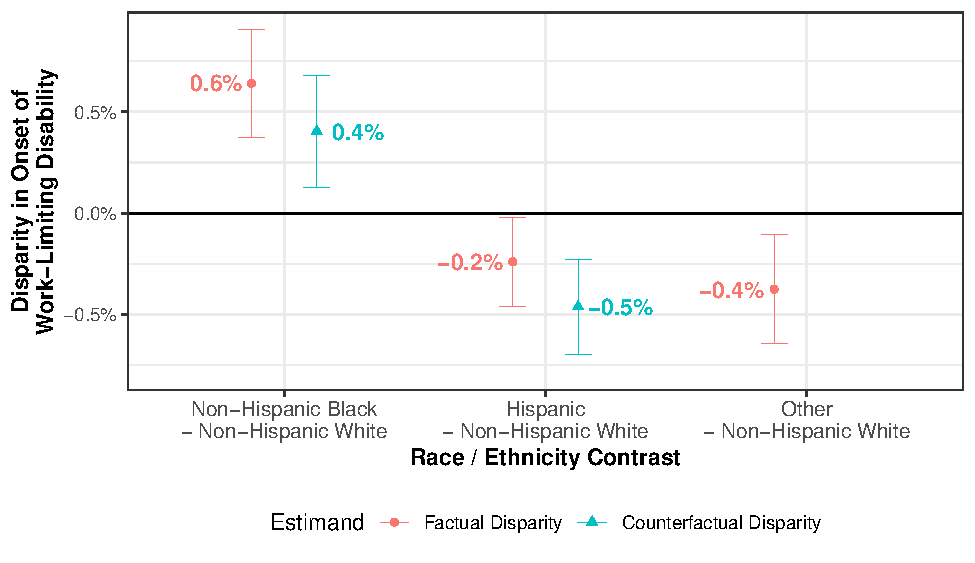
\includegraphics[width = \textwidth]{figures/disparity_6}};
    \node<10->[anchor = west] at (0,0) {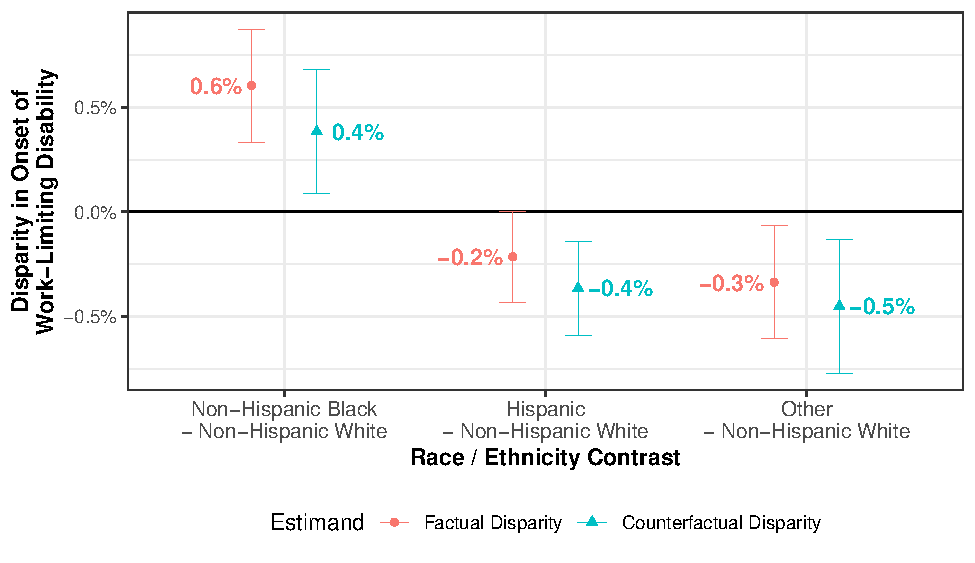
\includegraphics[width = \textwidth]{figures/disparity}};
    \node<4->[darkgray, font =  \scriptsize] at (.3,0) {37\% reduction};
    \draw<4->[->, thick, darkgray] (.3,.2) to[bend left] (.3, 1.1);
    \node<8->[darkgray, font =  \scriptsize, align = center] at (.57,1.7) {93\% increase\\in magnitude};
    \draw<8->[->, thick, darkgray] (.57,1.2) to[bend left] (.6, .5);
    \node<11->[darkgray, font =  \scriptsize, align = center] at (.85,1.7) {36\% increase\\in magnitude};
    \draw<11->[->, thick, darkgray] (.85,1.2) to[bend left] (.88, .5);
\end{tikzpicture}
\end{frame}

\begin{frame}%{How this is different}
\begin{tikzpicture}[x = \textwidth, y = \textheight]
\node at (0,0) {};
\node at (1,1) {};
\node<1->[anchor = north west, font = \bf, gray] at (0,.95) {Standard Regression};
\draw<2->[thick, rounded corners] (.137,.84) rectangle (.3,.89);
\node<1->[anchor = north west, font = \footnotesize] at (0,.9) {$\begin{aligned}Y = \beta_0 &+ \beta_1\times \texttt{Black} \\&+ \beta_2\times \texttt{College} \\&+ \beta_3\times \texttt{Lagged Health}\\&+ \beta_4\times \texttt{Occupation}\\&+(\texttt{other covariates})\\&+\epsilon\end{aligned}$};
\node<3->[anchor = north west, font = \bf, gray] at (.5,.95) {Gap-Closing Estimand};
\node<3->[align = center, font = \scriptsize] at (.63,.85) {Non-Hispanic Black};
\node<3->[align = center, font = \scriptsize] at (.89,.85) {Non-Hispanic white};
\node<3->[diamond, fill = lightgray, inner sep = 17pt] at (.63,.7) {};
\node<3->[align = center, font = \scriptsize] at (.63,.7) {Health if\\Occupations\\were Equitably\\Assigned};
\node<3-> at (.76,.7) {$-$};
\node<3->[circle, fill = lightgray, align = center, font = \scriptsize, inner sep = 0pt] at (.89,.7) {Health if\\Occupations\\were Equitably\\Assigned};
% Notes on each one
\node<4-5>[anchor = north, align = center, font = \footnotesize] at (0.25, .5) {Statistically holds\\\bgray{everything}\\equal};
\draw<4-5>[->, line width = 2pt, gray] (.25,.5) -- (.25,.55);
\node<5>[anchor = north, font = \footnotesize, align = center] at (0.75, .5) {An intervention\\to equalize\\\bgray{occupation}};
\draw<5>[->, line width = 2pt, gray] (.75,.5) -- (.75,.55);
%%%%%%%%%%%%%%%%%%%%%%%%
\node<6-18,21>[anchor = north west, font = {\bf\footnotesize}, gray, align = left, gray] (gce) at (.6,.52) {Gap-Closing Estimand};
\draw<6-18,21>[thick, gray] (gce.south west) -- (gce.south east);
\node<6-18,21>[anchor = north west, font = {\bf\footnotesize}, gray, align = left, gray] (sr) at (.2,.52) {Standard Regression};
\draw<6-18,21>[thick, gray] (sr.south west) -- (sr.south east);
\node<7-18,21>[anchor = north west, font = {\bf\footnotesize}, gray, align = left] at (0,.45) {Substantive\\Meaning};
\node<9-18,21>[anchor = north west, font = \footnotesize, align = left] at (.6,.45) {Outcome of an\\intervention};
\node<8-18,21>[anchor = north west, font = \footnotesize, align  = left] at (.2,.45) {Differences within\\subgroups};
\node<10-18,21>[anchor = north west, font = {\bf\footnotesize}, gray, align = left] at (0,.35) {Choice of\\Covariates};
\node<12-18,21>[anchor = north west, align = left, font = \footnotesize] at (.6,.35) {Those needed to identify\\the effect of occupation};
\node<11-18,21>[anchor = north west] at (.3,.35) {?};
\node<13-18,21>[anchor = north west, font = {\bf\footnotesize}, gray, align = left] at (0,.25) {Machine\\learning};
\node<15-18,21>[anchor = north west, align = left, font = \footnotesize] at (.6,.25) {Plug in\\and go!};
\node<14-18,21>[anchor = north west] at (.3,.25) {?};
\node<16-18,21>[anchor = north west, font = {\bf\footnotesize}, gray, align = left, gray] at (0,.15) {Policy\\Relevance};
\node<18,21>[anchor = north west, align = left, font = \footnotesize] at (.6,.15) {Speaks to the initial\\response to policy};
\node<17-18,21>[anchor = north west] at (.3,.15) {?};
\node<19>[anchor = north, draw, gray, line width = 2pt, rounded corners] at (.5,.52) {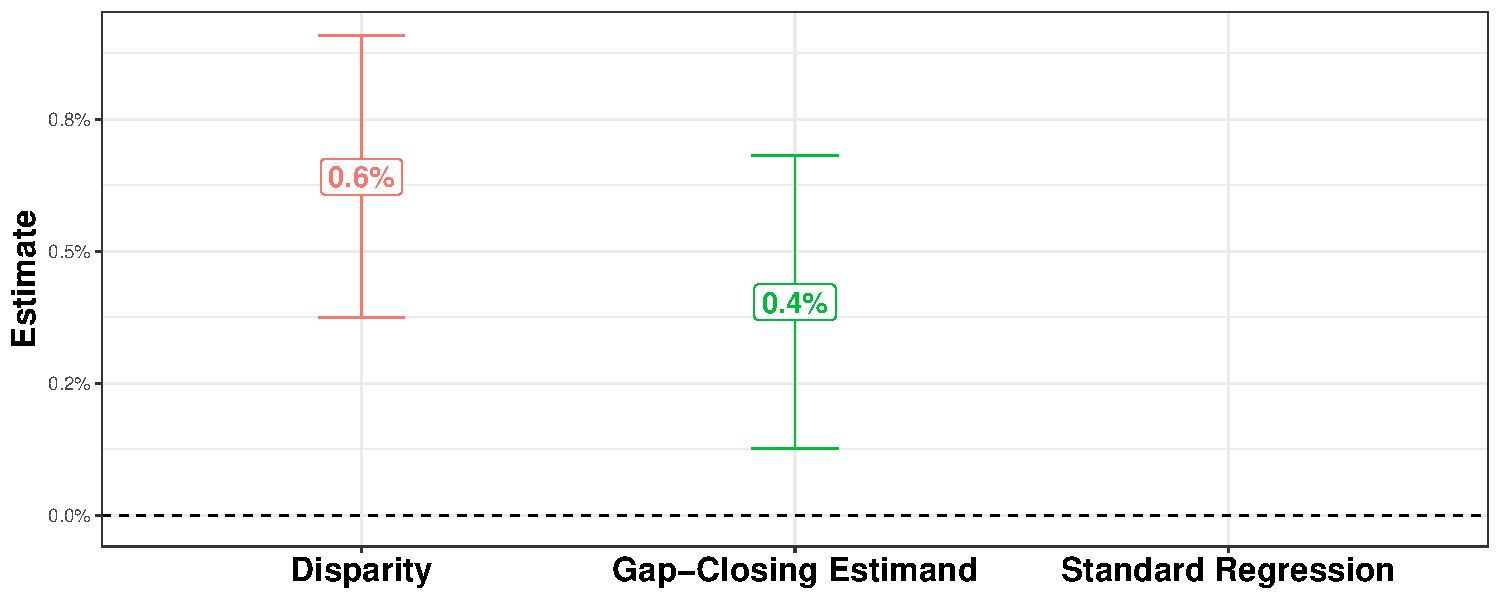
\includegraphics[width = .9\textwidth]{figures/conditional_gap_comparison_blackwhite_0}};
\node<20>[anchor = north, draw, gray, line width = 2pt, rounded corners] at (.5,.52) {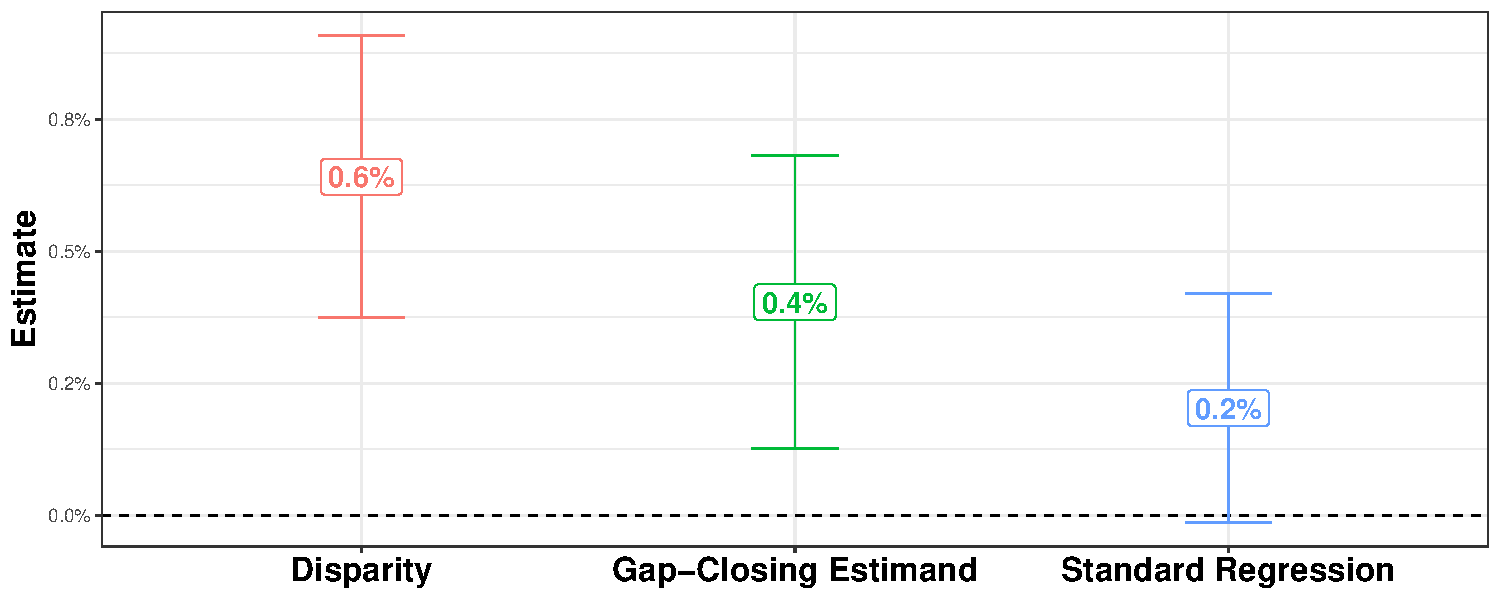
\includegraphics[width = .9\textwidth]{figures/conditional_gap_comparison_blackwhite}};
\end{tikzpicture}
\end{frame}

\begin{frame}
\begin{tikzpicture}[x = \textwidth, y = \textheight]
\node at (0,0) {};
\node at (1,1) {};
\node[anchor = north west, font = \large] at (0,.95) {\bblue{What we can do} that we could not do before};
\node<2->[anchor = north west] at (0,.83) {Place \bblue{race in a causal framework} with real people};
\node<3->[anchor = north west, font = \footnotesize, align = left] at (.1,.75) {Contrast:};
\node<3->[anchor = north west, font = \footnotesize, align = left] at (.25,.75) {Audit studies place race in a causal framework\\but with fictitious people};
\node<4->[anchor = north west, font = \footnotesize, align = left] at (.1,.65) {Contrast:};
\node<4->[anchor = north west, font = \footnotesize, align = left] at (.25,.65) {Disparities involve real people\\but without a causal framework};
\node<5->[anchor = north west] at (0,.53) {Produce evidence to inform \bblue{local policy interventions}};
\node<6->[anchor = north west, font = \footnotesize, align = left] at (.1,.45) {Contrast:};
\node<6->[anchor = north west, font = \footnotesize, align = left] at (.25,.45) {Structural claims (e.g.~eliminate dangerous jobs)\\are empirically intractable};
\node<7->[anchor = north west] at (0,.33) {Discover \bblue{treatment assignment rules} that close disparities};
\node<8->[anchor = north west, font = \footnotesize, align = left] at (.1,.25) {Contrast:};
\node<8->[anchor = north west, font = \footnotesize, align = left] at (.25,.25) {Precision medicine searches for effective\\person-specific treatments};
\node<9->[anchor = north west, font = \footnotesize, align = left] at (.25,.15) {The treatments that are effective to close\\population disparities might be different};
\end{tikzpicture}
\end{frame}

% Structure of the talk
\begin{frame}
\begin{tikzpicture}[x = \textwidth, y = \textheight]
\node at (0,0) {};
\node at (1,1) {};
\node[anchor = west, align = left] (gce) at (0.2, .9) {The \bblue{gap-closing estimand}:};
\node[anchor = west, align = left] (categories) at (0.2,.85) {The disparity across \bgreen{social categories}};
\node[anchor = west, align = left] (treatment) at (0.2,.8) {that would persist if we \bgreen{equalized a treatment}};
\node[anchor = east, align = right] at (.15, .88) {\bgray{General}};
\node[anchor = east, align = right] at (.15, .83) {\bgray{method}};
\draw[line width = 2pt, gray, line cap = round] (.175,.78) -- (.175,.93);
\node[anchor = west, align = left] (gce) at (.2, .7) {Occupational segregation contributes};
\node[anchor = west, align = left] (categories) at (.2,.65) {to racial disparities in health};
\node[anchor = east, align = right] at (.15, .7) {\bgray{Specific}};
\node[anchor = east, align = right] at (.15, .65) {\bgray{example}};
\draw[line width = 2pt, gray, line cap = round] (.175,.73) -- (.175,.63);
\node (plan) at (.5,.53) {\bgray{Structure of the talk}};
\draw[line width = 2pt, gray, line cap = round] (plan.south west) -- (plan.south east);
\node[anchor = west] at (.04,.44) {\bgray{Introduction}};
\node[anchor = west] at (.04,.38) {\bgray{Causal Question}};
\node[anchor = west] at (.04,.32) {\bgray{Estimation}};
\node[anchor = west] at (.04,.26) {\bgray{Results}};
\node[anchor = west] at (.04,.2) {\bgray{Broadening out}};
\node[anchor = west] at (.35,.44) {Approaches to understand disparities};
\node[anchor = west] at (.35,.38) {How an intervention would close a gap};
\node[anchor = west] at (.35,.32) {Causal assumptions and predictive tools};
\node[anchor = west] at (.35,.26) {Partially closing a gap in health};
\node[anchor = west] at (.35,.2) {A framework for quantitative methodology};
\draw[->, line width = 2pt, gray] (0,.26) -- (.04, .26);
\end{tikzpicture}
\end{frame}

\section{Discussion}

% Structure of the talk
\begin{frame}
\begin{tikzpicture}[x = \textwidth, y = \textheight]
\node at (0,0) {};
\node at (1,1) {};
\node[anchor = west, align = left] (gce) at (0.2, .9) {The \bblue{gap-closing estimand}:};
\node[anchor = west, align = left] (categories) at (0.2,.85) {The disparity across \bgreen{social categories}};
\node[anchor = west, align = left] (treatment) at (0.2,.8) {that would persist if we \bgreen{equalized a treatment}};
\node[anchor = east, align = right] at (.15, .88) {\bgray{General}};
\node[anchor = east, align = right] at (.15, .83) {\bgray{method}};
\draw[line width = 2pt, gray, line cap = round] (.175,.78) -- (.175,.93);
\node[anchor = west, align = left] (gce) at (.2, .7) {Occupational segregation contributes};
\node[anchor = west, align = left] (categories) at (.2,.65) {to racial disparities in health};
\node[anchor = east, align = right] at (.15, .7) {\bgray{Specific}};
\node[anchor = east, align = right] at (.15, .65) {\bgray{example}};
\draw[line width = 2pt, gray, line cap = round] (.175,.73) -- (.175,.63);
\node (plan) at (.5,.53) {\bgray{Structure of the talk}};
\draw[line width = 2pt, gray, line cap = round] (plan.south west) -- (plan.south east);
\node[anchor = west] at (.04,.44) {\bgray{Introduction}};
\node[anchor = west] at (.04,.38) {\bgray{Causal Question}};
\node[anchor = west] at (.04,.32) {\bgray{Estimation}};
\node[anchor = west] at (.04,.26) {\bgray{Results}};
\node[anchor = west] at (.04,.2) {\bgray{Broadening out}};
\node[anchor = west] at (.35,.44) {Approaches to understand disparities};
\node[anchor = west] at (.35,.38) {How an intervention would close a gap};
\node[anchor = west] at (.35,.32) {Causal assumptions and predictive tools};
\node[anchor = west] at (.35,.26) {Partially closing a gap in health};
\node[anchor = west] at (.35,.2) {A framework for quantitative methodology};
\draw[->, line width = 2pt, gray] (0,.2) -- (.04, .2);
\end{tikzpicture}
\end{frame}

\begin{frame}
\begin{tikzpicture}[x = \textwidth, y = \textheight]
\node at (0,0) {};
\node at (1,1) {};
%\node[anchor = west, align = left] at (0,.9) {Quantitative methods are all about \bblue{estimating quantities}\\that answer \bblue{precise questions} motivated by theory.};
\node<2-6>[anchor = west] at (0,.95) {What we want:};
\node<2->[cloud, draw, align=center, cloud puffs=20,cloud puff arc=110, aspect=2, inner sep=.5mm] (theory) at (.25,.8) {Theoretical\\question};
\node<3->[align = center] (data) at (.75,.8) {Things we do\\to data};
\draw<3->[->, line width = 3pt, gray] (theory) -- node[midway, above, font = \bf] {motivate} (data);
\node<4-6>[anchor = west] at (0,.6) {What actually happens:};
\node<5-6>[align = center] (familiar_methods) at (.75,.5) {Familiar methods\\(regression)};
\node<6>[align = center] (questions_we_ask) at (.25,.5) {Questions\\we ask};
\draw<6>[->, line width = 3pt, red] (familiar_methods) -- node[midway, above, font = \bf] {constrain} (questions_we_ask);
%\node<7>[align = center] at (.5, .25) {But regression coefficients are only\\\bblue{one small slice}\\of all the theoretical questions we could ask};
\node<8->[align = left, font = \small, anchor = south west, gray] at (0,0.05) {Lundberg, Johnson, Stewart\\\textbf{What is Your Estimand?}\\Defining the Target Quantity Connects Statistical Evidence to Theory\\Forthcoming, \emph{American Sociological Review}};
% Begin the proposed estimand statement
\node<9->[circle, fill = lightgray, draw = lightgray, font = \footnotesize, inner sep = 8pt] (point1) at (.65,.6) {};
\node<10>[font = \scriptsize] at (point1) {$Y_i$};
\node<11->[font = \scriptsize] at (point1) {$Y_i(t)$};
\node<9->[gray, font = \footnotesize, align = center, anchor = north] (usqNote) at (point1.south) {A \bgray{unit-specific}\\\bgray{quantity}};
\node<12->[circle, fill = lightgray, draw = lightgray, font = \footnotesize, inner sep = 8pt] (point2) at (.78,.55) {};
\node<12->[circle, fill = lightgray, draw = lightgray, font = \footnotesize, inner sep = 8pt] (point3) at (.7,.4) {};
\node<12->[circle, fill = lightgray, draw = lightgray, font = \footnotesize, inner sep = 8pt] (point4) at (.85,.43) {};
\node<12->[circle, fill = lightgray, draw = lightgray, font = \footnotesize, inner sep = 8pt] (point5) at (.58,.42) {};
\node<12->[circle, fill = lightgray, draw = lightgray, font = \footnotesize, inner sep = 8pt] (point6) at (.9,.6) {};
\draw<12->[line width = 2pt, gray, rounded corners] (.53,.33) rectangle (.95,.67);
\node<12->[gray, font = \footnotesize, align = center, anchor = north] at (.74,.33) {Aggregated over a\\\bgray{target population}};
\node<12->[font = \scriptsize] at (point1) {$Y_i(t)$};
\node<12-17>[font = \scriptsize] at (point2) {$Y_i(t)$};
\node<12->[font = \scriptsize] at (point3) {$Y_i(t)$};
\node<12-17>[font = \scriptsize] at (point4) {$Y_i(t)$};
\node<12-17>[font = \scriptsize] at (point5) {$Y_i(t)$};
\node<12->[font = \scriptsize] at (point6) {$Y_i(t)$};
\node<13->[anchor = north west, align = left] (caption1) at (0,.57) {Our framework expands \bblue{theory},};
\node<13->[anchor = north west, align = left] (caption2) at (caption1.south west) {links to transparent \bblue{evidence},};
\node<13->[anchor = north west, align = left] at (caption2.south west) {and unlocks computational \bblue{tools}};
\draw<14>[line width = 2pt, blue] (.375,.51) -- (.48,.51);
\draw<15-16>[line width = 2pt, blue] (.31,.445) -- (.46,.445);
\draw<17->[line width = 2pt, blue] (.425,.38) -- (.503,.38);
\node<16->[circle, draw = black, font = \footnotesize, inner sep = 8pt, line width = 2pt] at (point1) {};
\node<16->[circle, draw = black, font = \footnotesize, inner sep = 8pt, line width = 2pt] at (point3) {};
\node<16->[circle, draw = black, font = \footnotesize, inner sep = 8pt, line width = 2pt] at (point6) {};
\node<18>[font = \scriptsize] at (point2) {$\hat{Y}_i(t)$};
\node<18>[font = \scriptsize] at (point4) {$\hat{Y}_i(t)$};
\node<18>[font = \scriptsize] at (point5) {$\hat{Y}_i(t)$};
\end{tikzpicture}
\end{frame}

% Closing slide
\begin{frame}
\begin{tikzpicture}[x = \textwidth, y = \textheight]
\node at (0,0) {};
\node at (1,1) {};
% BRING BACK GAP-CLOSING
\node[font = \footnotesize, anchor = north east,align  = right] at (.3,.4) {\bgray{The gap-closing}\\\bgray{estimand}};
\node[font = \footnotesize, anchor = north west,align  = left] at (.35,.4) {A causal approach to study interventions\\that close disparities across social categories};
\node[font = \footnotesize] at (.15, .11) {\bgray{Categories}};
\node[font = \footnotesize] at (.45, .11) {\bgray{Treatment}};
\node[font = \footnotesize, align = center] at (.8, .11) {\bgray{Counterfactual Disparity}};
\node[circle, fill = lightgray, draw = lightgray, font = \footnotesize, inner sep = 2pt] at (.11,.25) {\phantom{$t$}};
\node[circle, fill = lightgray, draw = lightgray, font = \footnotesize, inner sep = 2pt] at (.11,.17) {\phantom{$t$}};
\node[diamond, fill = lightgray, draw = lightgray, font = \footnotesize, inner sep = 2pt] at (.19,.25) {\phantom{$t$}};
\node[diamond, fill = lightgray, draw = lightgray, font = \footnotesize, inner sep = 2pt] at (.19,.17) {\phantom{$t$}};
\node[circle, fill = lightgray, draw = lightgray, font = \footnotesize, inner sep = 2pt] at (.41,.25) {$t$};
\node[circle, fill = lightgray, draw = lightgray, font = \footnotesize, inner sep = 2pt] at (.41,.17) {$t$};
\node[diamond, fill = lightgray, draw = lightgray, font = \footnotesize, inner sep = 2pt] at (.49,.25) {$t$};
\node[diamond, fill = lightgray, draw = lightgray, font = \footnotesize, inner sep = 2pt] at (.49,.17) {$t$};
\node[circle, fill = lightgray, draw = lightgray, font = \footnotesize, inner sep = 2pt] at (.73,.21) {$\bar{y}(t)$};
\node[font = \footnotesize] at (.8,.21) {$-$};
\node[diamond, fill = lightgray, draw = lightgray, font = \footnotesize, inner sep = 2pt] at (.88,.21) {$\bar{y}(t)$};
\node[align = center] at (.5,.7) {\textbf{Ian Lundberg}\\\href{https://www.ianlundberg.org/}{\blue{ianlundberg.org}}}; 
%\node<22->[align = right, anchor = east] at (1,.7) {Replication code on GitHub\\Slides on GitHub\\Drafts}; 
\end{tikzpicture}
\end{frame}

\end{document}
